\documentclass[11pt,oneside]{report}

\usepackage{graphicx}
\graphicspath{{LateX images/}}
\usepackage[hidelinks]{hyperref} 
\usepackage{caption}
\usepackage{subcaption}
\usepackage{titlesec}
\titleformat{\chapter}[display]
{\normalfont\bfseries}{}{0pt}{\Huge}
\usepackage{fontspec}
\setmainfont[Scale=0.76]{Roboto}
\setsansfont[Scale=0.76]{Roboto}
\newfontfamily{\greekfont}{Roboto}
\newfontfamily{\greekfontsf}{Roboto}
\usepackage{polyglossia}
\setdefaultlanguage{greek}
\usepackage[a4paper,width=150mm,top=25mm,bottom=25mm,bindingoffset=6mm]{geometry}
\usepackage{fancyhdr}
\pagestyle{fancy}
\fancyhf{}
\fancypagestyle{plain}{}
%\fancyhead[LE,RO]{Thesis title}
%\fancyhead[RE,LO]{\leftmark}
%\fancyfoot[LO,RE]{Βασίλειος Ασημακόπουλος}
%\fancyfoot[LE,RO]{\thepage}
\renewcommand{\headrulewidth}{0.4pt}
\renewcommand{\footrulewidth}{0.4pt}
\renewcommand{\figurename}{Fig.}
\makeatletter 
\renewcommand{\thesubfigure}{\@roman\c@subfigure}
\makeatother

\title{
	{okoko}\\
	{\large asdasda}\\
	
	{
\includegraphics{AUTH_main_logo.png}}
}
\author{Βασίλειος Ασημακόπουλος}
\date{16/05/2022}

\begin{document}

\maketitle
\chapter*{Ευχαριστίες}


\chapter*{Περίληψη}


\chapter*{Abstract}


\tableofcontents{}

\chapter{Κεφάλαιο 1}
Στο συγκεκριμένο κεφάλαιο παρουσιάζεται το θεωρητικό υπόβαθρο πάνω στο οποίο βασίστηκε η μελέτη στα πλαίσια της παρούσας πτυχιακής εργασίας.
Ειδικότερα, παρουσιάζονται η απαραίτητη θεωρία των μη-γραμμικών δυναμικών συστημάτων, τα εργαλεία που χρησημοποιήθηκαν για την μελέτη των συστημάτων, όπως και τα φαινόμενα που παρατηρήθηκαν κατά την διάρκεια της μελέτης.

\section{Δυναμικά Συστήματα}

Δυναμικά συστήματα ονομάζονται τα φυσικά συτήμτα και οι φυσικές διεργασίες που περιγράφονται απο συστήματα είτε διαφορικων εξισώσεων είτε εξισώσεων διαφορών , των οποίων ανεξάρτητη μεταβλητή ειναι ο χρόνος \cite{b1}.

Αν θεωρήσουμε ένα Ν-διάστατο χώρο εξαρτημένων μεταβλητών $x_k(t)$, με $k =1, 2, ...., N$, που έχουν ώς μόνη ανεξάρτητη μεταβλητή τους το χρόνο  $t$ και αποτελούν συνιστώσες του διανύσματος:

\begin{equation}	
	x (t)= \bigl( x_1(t) , x_2(t), .... , x_N(t) \bigl) ,\quad t \in I= (α,β)
	\label{m:g1}
\end{equation}

όταν ο χρόνος είναι \textbf{συνεχής} στο διάστημα \textbf{I} (οι μεταβλητές θεωρούνται πραγματικές) ή ενός διανύσματος:

\begin{equation}	
	x_n = x(t_n)= \bigl( x_{1,n}, x_{2,n}, .... , x_{N,n} \bigl) , \quad x(k_n)= x_k(t_n)
	\label{m:g2}
\end{equation}

όταν ο χρόνος παίρνει \textbf{διακριτές} τιμές $t_n$ ($n$ ακέραιος).
Η εξέλιξη στο χρόνο των διανυσμάτων αυτών, δίνεται απο ένα σύστημα 
\emph{διαφορικών εξισώσεων} πρώτης τάξης αν το $t$ είναι συνεχές :
\begin{equation}
	\frac{d\textbf{x}}{dt} = \textbf{x} = \textbf{f}(\textbf{x},t)  \quad  \text{ή} \quad  
	x_k = f_k (\textbf{x},t), \quad k=1,2, .... , N ,
	\label{m:g3}
\end{equation}

ή ένα σύστημα εξισώσεων διαφορών

\begin{equation}	
	x_{n+1} = \textbf{g}(\textbf{x}_n), \quad \text{ή}  \quad x_{k,n+1}= g_k(\textbf{x}_n), \quad k=1,2, .... , N
	\label{m:g4}
\end{equation}

αν $t$ διακριτό και ορίζεται ως το δυναμικό σύστημα που περιγράφει το φυσικό φαινόμενο που μας ενδιαφέρει. Οι διανυσματικές συναρτήσεις \textbf{f} και \textbf{g} αποτελούν την "μαθητικοποίηση"
του φαινομένου και φυσικά διαφέρουν ανάλογα με τους φυσικούς νόμους που διέπουv κάθε φαινόμενο. Ο Ευκλείδιος χώρος $ \mathbb{R} ^Ν$ στον οποίον εξελίσσονται τα διανύσματa $\textbf{x}(t)$ και $\textbf{x}(n)$ λέγεται \textbf{χώρος φάσεων του συστήματος} \cite{b1}.

\newpage

Συμβολικά, λοιπόν, μπορούμε να ορίσουμε ένα δυναμικό σύστημα ως μια \textbf{ροή} (ή απεικόνιση)  $φ(x,t)$  στο χώρο φάσεων:
\begin{equation}
	φ: R\times E \to E ,
\end{equation}
η οποία μεταφέρει (ή απεικονίζει) ένα σημείο $\textbf{x}=(x_1,x_2,....,x_n)$ , το οποίο αντιστοιχεί στη θέση του
συστήματος τη χρονική στιγμή $t$, σε ένα
σημείο $\textbf{x'}=(x_1,x_2,....,x_n)$, το οποίο αντιστοιχεί στη θέση του συστήματος τη χρονική στιγμή $t'$,

\begin{equation}
	\textbf{x}=φ(x,t)
\end{equation}

Μια ροή έχει τις ιδιότητες:

\begin{gather}
	φ(\textbf{x},0)=\textbf{x} \\
	φ(φ(\textbf{x},t_1),t_2)=φ(\textbf{x},t_1+t_2)
\end{gather}
Μπορούμε να ορίσουμε τη θέση $x_0 = (x_{10}, x_{20},...., x_{n0})$ σε μια χρονική στιγμή $t_0$ ως την αρχική θέση του
συστήματος. Αρχική θέση για το σύστημα μπορεί να αποτελεί κάθε σημείο του χώρου των φάσεων και η ροή $φ(x,t)$ του δυναμικού συστήματος μπορεί να εφαρμοστεί σε οποιαδήποτε αρχική θέση του συστήματος. Εν γένει, η εξέλιξη του συστήματος που αντιστοιχεί σε διαφορετική αρχική θέση είναι επίσης διαφορετική. Αν ο κανόνας εξέλιξης που εκφράζεται με την ροή δεν εμπλέκει «τυχαιότητα» τότε το σύστημα ονομάζεται \textbf{αιτιοκρατικό} (deterministic). Ένα αιτιοκρατικό σύστημα δίνει πάντα την ίδια εξέλιξη για μια δοθείσα αρχική θέση. Αν η ροή συμπεριλαμβάνει κάποιον βαθμό τυχαιότητας με τον ορισμό πιθανοτήτων στον κανόνα της εξέλιξης τότε το σύστημα ονομάζεται \textbf{στοχαστικό} (stochastic). 

Αν η ροή $φ(x,t)$ ενός αιτιοκρατικού συστήματος δεν εξαρτάται ρητά από το χρόνο $t$ τότε το σύστημα ονομάζεται αυτόνομο. Σε ένα τέτοιο σύστημα, η εξέλιξη του συστήματος είναι ανεξάρτητη από την αρχική
χρονική στιγμή. Αντίθετα, σε ένα μη-αυτόνομο σύστημα, αν το σύστημα βρεθεί σε ένα σημείο $x \in E$, η εξέλιξή του στο χρόνο εξαρτάται και από την χρονική στιγμή t στην οποία βρίσκεται στο \textbf{x}.

Αν και στη φύση ο χρόνος $t$ αποτελεί μια συνεχή μεταβλητή, σε ένα δυναμικό σύστημα ο χρόνος μπορεί να είναι συνεχής ή διακριτός \cite{b2}.


\subsection{Συνεχές Δυναμικό Σύστημα}

Στην πρώτη περίπτωση ο χρόνος μπορεί να πάρει μια οποιαδήποτε πραγματική τιμή και το δυναμικό σύστημα ονομάζεται \textbf{συνεχές} \cite{b2}.

\subsection{Διακριτό Δυναμικό Σύστημα}
Αν όμως η εξέλιξη του συστήματος περιγράφεται σε χρονικά βήματα ανά $Δt$, τότε ο χρόνος παίρνει τις διακριτές τιμές $t_k = t_0 + kΔt$ και το σύστημα ονομάζεται \textbf{διακριτό} (discrete). 
Για ένα διακριτό σύστημα μια χρονική στιγμή $t \in(t_k,t_{k+1}) $ δεν έχει νόημα \cite{b2}.

Στη συγκεκριμένη εργασία όλα τα συστήματα που μελετήθηκαν ανήκουν στην κατηγορία των διακριτών, μη - γραμμικών συστημάτων.

\clearpage

\section{Χαοτικά Συστήματα}

Τα χαοτικά συστήματα αποτελούν μια ξεχωριστή αυτοδύναμη κατηγορία δυναμικών συστημάτων. Αν και φαίνονται στοχαστικά όταν παρατηρούνται, παρ’ όλα αυτά περιγράφονται μαθηματικά από μη γραμμικές διαφορικές εξισώσεις (ροές) ή από μη
γραμμικές εξισώσεις διαφορών (απεικονίσεις) και ανήκουν στην κατηγορία των μη γραμμικών αιτιοκρατικών συστημάτων. Η τροχιά τους για ένα σύνολο αρχικών συνθηκών, περιορίζεται σε ένα υποχώρο του χώρου φάσεων που στην προκειμένη περίπτωση επειδή εμφανίζει πρωτότυπες (παράξενες) ιδιότητες λέγεται παράξενος ελκυστής. Αν και ο χώρος που εξελίσσεται η τροχιά είναι περιορισμένος, αυτή δεν διέρχεται ποτέ από το ίδιο σημείο δύο φορές, δηλαδή δεν κόβει τον εαυτό της, έχει άπειρο μήκος, είναι απεριοδική και τούτο φαίνεται καθαρά στο φάσμα ισχύος μια μεταβλητής του συστήματος που είναι συνεχές. Επίσης φαίνεται να περιφέρεται τυχαία, δηλαδή οι μελλοντικές θέσεις της να μην σχετίζονται με τις παρελθούσες, για αυτό και ο συντελεστής αυτοσυσχέτισης μια μεταβλητής ενός χαοτικού συστήματος μηδενίζεται
σε σχετικά μικρό χρονικό διάστημα \cite{b3}.


\section{Χαοτικά Χαρακτηριστηκά}

\begin{enumerate}
	\item Το χαοτικό σύστημα πρέπει να είναι τοπολογικά μεταβατικό. 
	Τοπολογική μεταβατικότητα (ή τοπολογική ανάμειξη), σημαίνει ότι το
	σύστημα θα εξελιχθεί με την πάροδο του χρόνου, έτσι ώστε κάθε συγκεκριμένη
	περιοχή ή ανοιχτό σύνολο του χώρου φάσης τελικά θα συμπίπτει με οποιαδήποτε
	άλλη περιοχή. H ανάμειξη των έγχρωμων βαφών ή υγρών είναι ένα παράδειγμα ενός χαοτικού συστήματος \cite{b11}.
	\item Eυθαισθησία στις αρχικές συνθήκες.
	Το κύριο χαρακτηριστικό των χαοτικών συστημάτων, είναι η
	ευαίσθητη εξάρτηση από τις αρχικές συνθήκες. Δηλαδή, αν δοθούν δύο τυχαίες διαφορετικές αρχικές συνθήκες $x_1(0)$ και $x_2(0) = x_1(0) + Δt(0) $, η μια κοντά στην άλλη, οι τροχιές που προκύπτουν αποκλίνουν μέχρι να καταστούν ασυσχέτιστες \cite{b2}.
\end{enumerate}


\section{Εργαλεία μελέτης χαοτικών συστημάτων}
Τα βασικά εργαλεία που χρησιμοποιήθηκαν στην μελέτη της εργασίας αναλύονται στη συνέχεια.

\subsection{Διάγραμμα Διακλάδωσης}

Tα διαγράμματα διακλάδωσης χρησιμοποιούνται κυρίως για την ποιοτική μελέτη της ροής ενός χαοτικού συστήματος αλλάζοντας μία παράμετρο k. Συγκεκριμένα σημεία ισορροπίας μπορούν να δημιουργηθούν ή να καταστραφούν ή να αλλάξει η ευστάθεια τους. Τέτοιες ποιοτικές μεταβολές σε ένα σύστημα της ονομάζουμε \textbf{διακλαδώσεις} και οι τιμές των παραμέτρων κατά τις οποίες εμφανίζονται αυτές οι αλλαγές ονομάζονται \textbf{σημεία διακλάδωσης}. Στα διαγράμματα διακλάδωσης, παρατηρούμε τόσο χαοτικές όσο και περιοδικές περιοχές, ενώ στην περίπτωση που εξετάζουμε ένα χαοτικό σύστημα, παρατηρούνται φαινόμενα όπως ο \emph{διπλασιασμός περιόδου}, η \emph{υστέρηση}, η \emph{συνύπαρξη ελκυστών}, 
η \emph{αντιμονοτονικότητα} και η \emph{κρίση ελκυστών}, τα οποία θα αναλυθούν στην επόμενη παράγραφο \cite{b4}.

\subsection{Εκθέτης Lyapunov}
Ο εκθέτης Lyapunov μιας απεικόνισης αποτελεί ένα μέτρος της ευαισθησίας της εξάρτησης από τις αρχικές συνθήκες, η οποία είναι χαρακτηριστική της χαοτικής συμπεριφοράς ενός συστήματος. Ο εκθέτης Lyapunov (συμβολίζεται με \emph{λ}), μπορεί να υπολογιστεί για μία μονοδιάστατη απεικόνιση. Αν ένα σύστημα μπορεί να εξελιχθεί απο δύο διαφορετικές καταστάσεις , $x$ και $ x + ε_0$ τότε μετά απο $n$ επαναλήψεις η απόκλιση των δύο καταστάσεων δίνεται από τη σχέση

\begin{equation}
	ε(n) = ε_02^λn
\end{equation}

όπου ο εκθέτης Lyapunov λ δίνει τη μέση τιμή του ρυθμού απόκλισης. Αν ο λ είναι αρνητικός, τότε η εξέλιξη του συστήματος δεν οδηγεί σε χαοτική συμπεριφορά γιατί οι τροχιές συγκλίνουν. Αν ο λ είναι θετικός, τότε οι γειτονικές τροχιές αποκλίνουν, οπότε η εξέλιξη του συστήματος είναι ευαίσθητη στις αρχικές συνθήκες που είναι το κύριο χαρακτηριστηκό του χάους \cite{b5}.

\subsection{To διάγραμμα $x_i - x_{i+1}$}

Στο διάγραμμα $x_i - x_{i+1}$ απεικονίζονται οι λύσεις των εξισώσεων σε σχέση με τις προηγούμενες. Όταν ένα σύστημα είναι σε περίοδο - 1 σημαίνει ότι η εξίσωση παράγει συνέχεια μια λύση. Άρα αυτή και η προηγούμενη ταυτίζονται. Επομένως στο διάγραμμα βλέπουμε ένα σημείο. Όταν  ένα σύστημα είναι σε χάος σημαίνει ότι η εξίσωση παράγει άπειρες λύσεις. Επομένως στο διάγραμμα βλέπουμε άπειρα σημεία τα οποία σχηματίζουν μια καμπύλη. το πλήθος των σημείων στο διάγραμμα αντιστοιχεί στο πλήθος των λύσεων που παράγει η εκάστοτε εξίσωση.
\begin{figure}[ht]
	\centering
	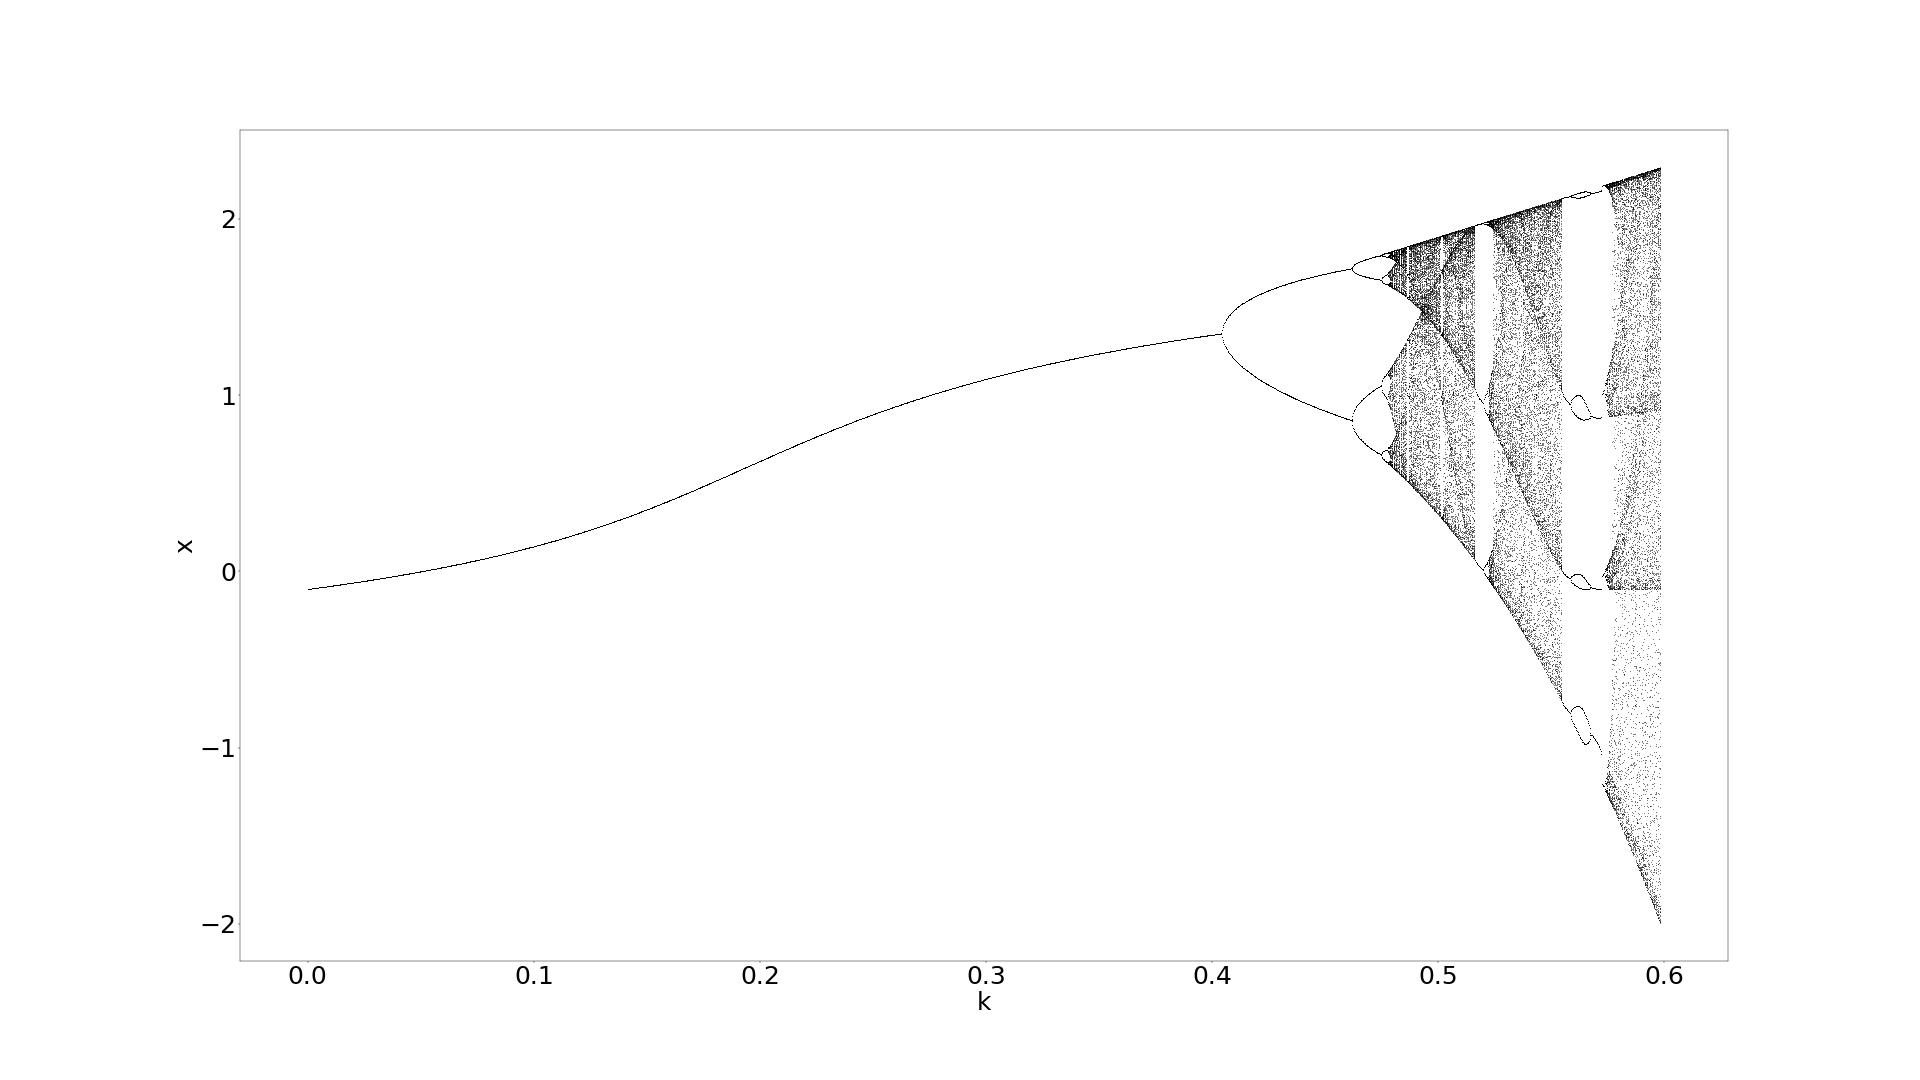
\includegraphics[width=1\linewidth]{LateX images/graphs/g1}
	\caption{ Διάγραμμα διακλάδωσης.}
	\label{th:g1}	
\end{figure}

\clearpage

\section{Φαινόμενα Χαοτικών Συστημάτων}
Τα φαινόμενα που θα αναλυθουν παρακάτω παρατηρήθηκαν στα συστήματα που μελετήθηκαν στα επόμενα κεφάλαια.

\subsection{Διπλασιασμός Περιόδου}

Αυτό το φαινόμενο παρατηρείται σε χαοτικά συστήματα όπως η λογιστική απεικόνιση. Ουσιαστικά οι διακλαδώσεις σε ένα διάγραμμα όπως στο Σχ. \ref{th:g1} όσο αυξάνεται η παράμετρος k διπλασιάζονται απο περίοδο-1 σε περίοδο-2 μέχρι που για συγκεκριμένο k το σύστημα εισέρχεται σε χάος \cite{b5}.

\subsection{Υστέρηση}
Όταν μεταξύ των ορίων διαφόρων περιοδικών περιοχών υπάρχει ασυνέχεια, τότε αυτό ονομάζεται φαινόμενο υστέρησης.

\subsection{Κρίση Ελκυστών}

Όταν παρατηρούμε μία απότομη ασυνεχή μεταβολή σε ένα χαοτικό ελκυστή
ενώ μεταβάλλεται μία παράμετρος του συστήματος,το ονομάζουμε κρίση ελκυστών. 
Οι ασυνεχείς μεταβολές είναι τυπικά τριών τύπων \cite{b5} :
\begin{enumerate}
	\item Ένας χαοτικός ελκυστής καταστρέφεται καθώς η παράμετρος περνά από μια κρίσιμη τιμή.Το είδος αυτής της κρίσης ονομάζεται συνοριακή κρίση (boundary crisis).
	\item Το μέγεθος του χαοτικού ελκυστή στο χώρο των φάσεων αυξάνεται ξαφνικά καθώς η παράμετρος περνά από την κρίσιμη τιμή της. Το είδος αυτής της κρίσης ονομάζεται
	εσωτερική κρίση, καθώς ο ελκυστής συγκρούεται με μία περιοδική τροχιά στο εσωτερικό της δεξαμενής έλξης του.
	\item Δύο ή περισσότεροι ελκυστές συγχωνεύονται για να σχηματίσουν ένα χαοτικό ελκυστή. 
\end{enumerate}
Το αντίστροφο αυτών των διαδικασιών επίσης συμβαίνουν καθώς η παράμετρος ελέγχου περνά από την κρίσιμη τιμή, κατά την αντίθετη κατεύθυνση.

\subsection{Aντιμονοτονικότητα}
Το φαινόμενo της αντιμονοτονικοτητας μπορει να εμφανιστεί με δύο τρόπους \cite{b5} :
\begin{enumerate}
	
	\item Μπορεί να παρατηρηθεί σε ένα διάγραμμα διακλάδωσης κατά την αύξηση της παραμέτρου k όταν το σύστημα ενώ μπαίνει με διπλασιασμό περιόδου στο χάος, στη συνέχεια εξέρχεται από αυτό με μία ανάστροφη ακολουθία διπλασιασμού της περιόδου και έτσι το σύστημα καταλήγει στην αρχική περίοδο του. Το σχήμα που προκύπτει στο διάγραμμα διακλάδωσης ονομάζεται χαοτική φυσαλίδα. Αυτό μπορεί να παρατηρηθεί στο Σχ. \ref{th:g3}.
	
	\item  Καθώς μεταβάλλεται η παράμετρος k, μεταξύ δύο χαοτικών περιοχών παρατηρείται μια ανάστροφη ακολουθία διπλασιασμού της περιόδου μέχρι να φτάσει σε περίοδο-1 και στη συνέχεια με διπλασιασμό της περιόδου καταλήγει πάλι στο χάος.Αυτό μπορεί να παρατηρηθεί στο Σχ. \ref{th:g4}.
	
\end{enumerate}


\subsection{Συνύπαρξη ελκυστών}
Το φαινόμενο της συνύπαρξης ελκυστών είναι το φαινόμενο κατά το οποίο το σύστημα για διαφορετικές αρχικές συνθήκες παρουσιάζει εντελώς διαφορετική δυναμική συμπεριφορά \cite{b5}.

\begin{figure}[ht]
	\centering
	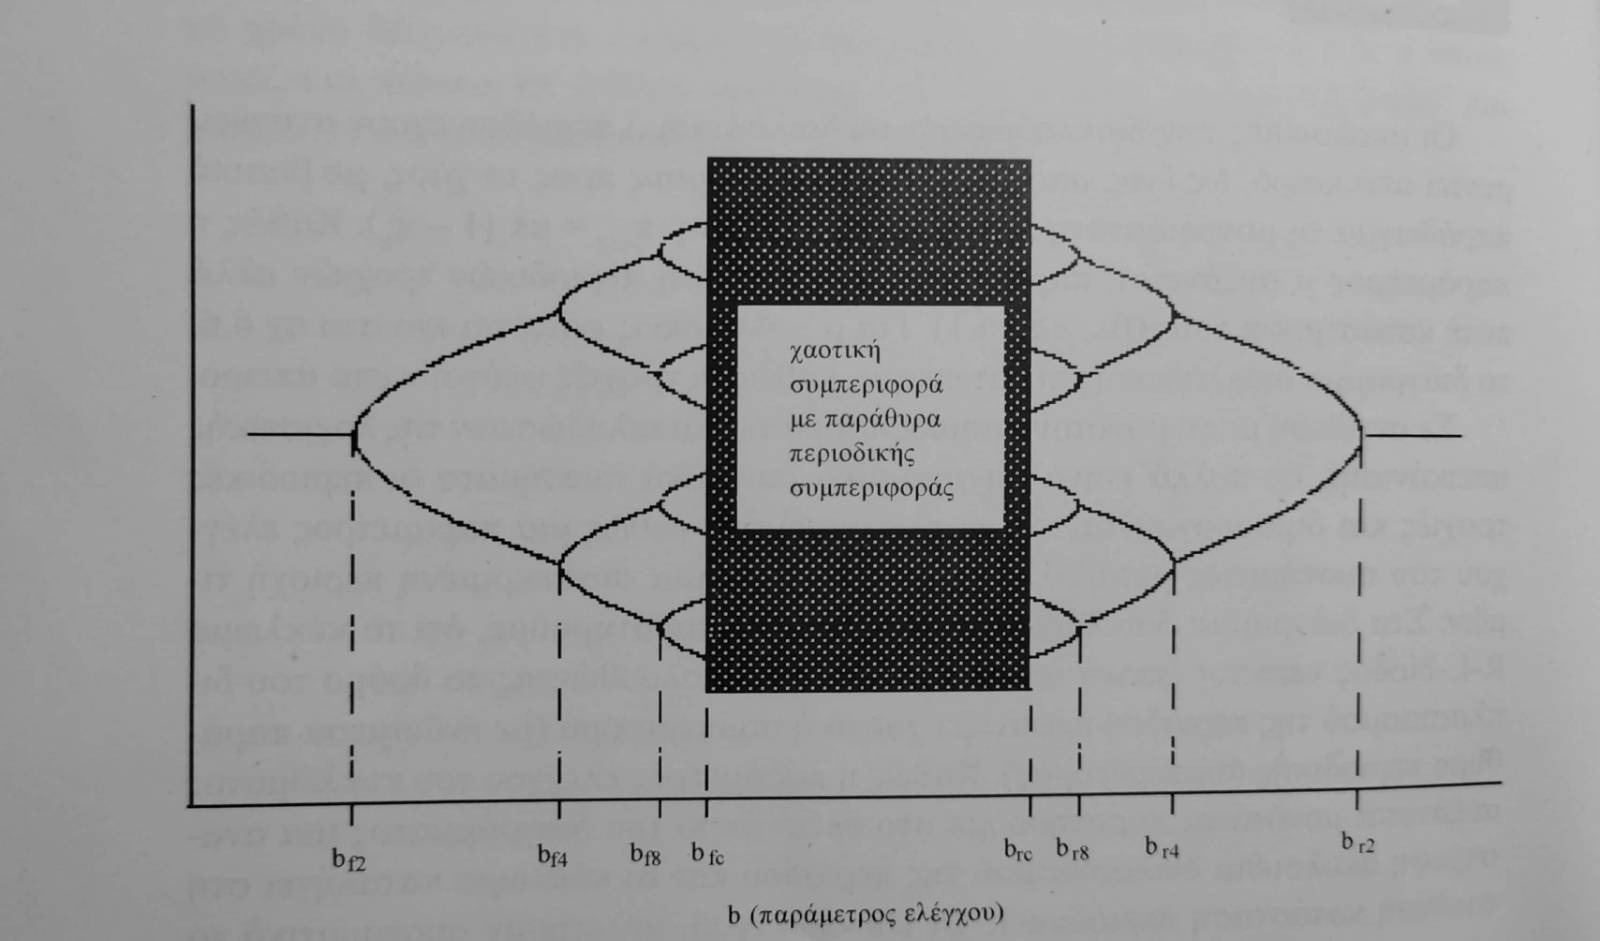
\includegraphics[width=1\linewidth]{LateX images/antimon1}
	\caption{ Σχηματικό διάγραμμα φυσαλίδας περιόδου-1.}
	\label{th:g3}	
\end{figure}

\begin{figure}[ht]
	\centering
	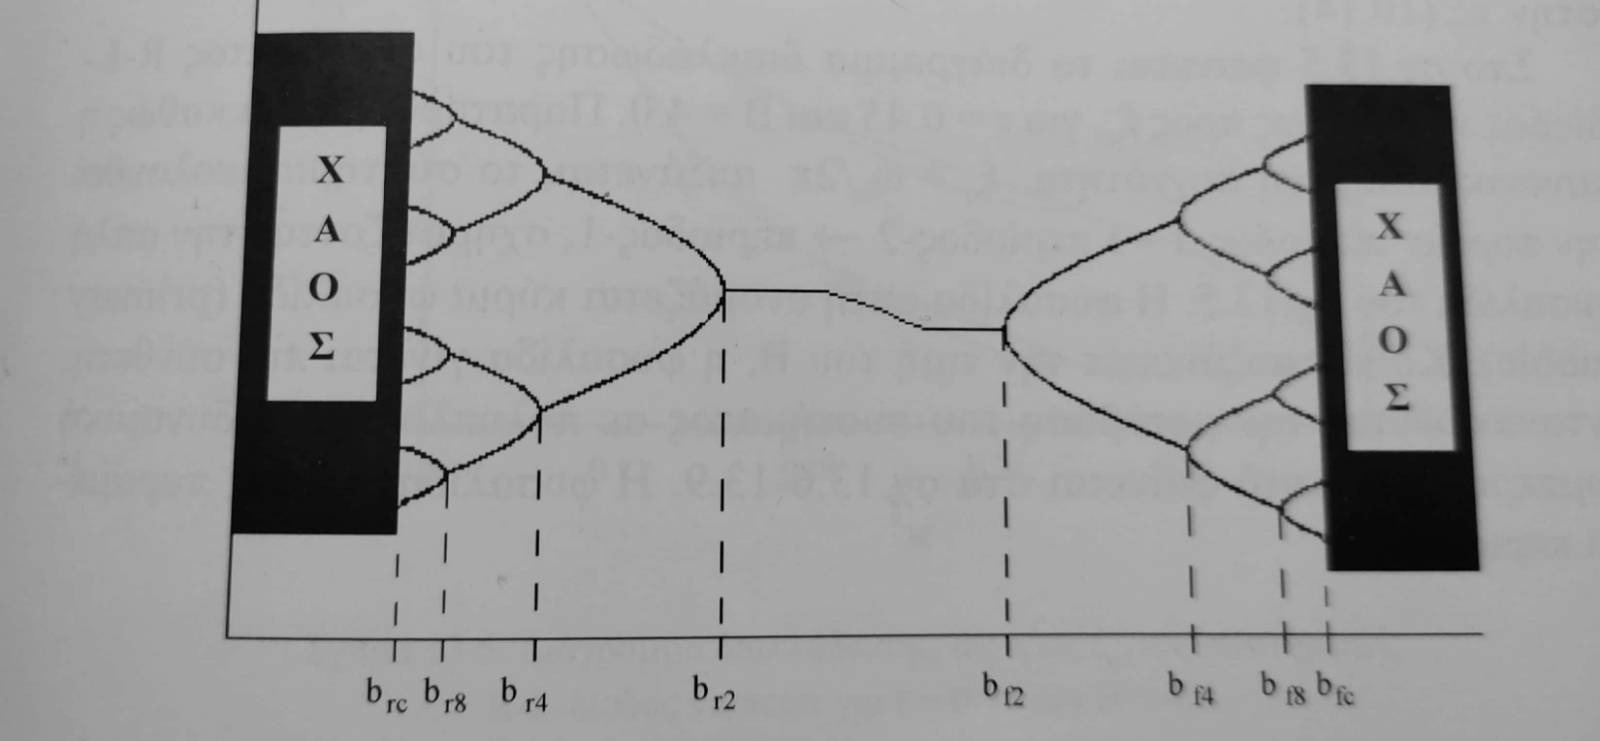
\includegraphics[width=1\linewidth]{LateX images/antimon2}
	\caption{ Σχηματικό διάγραμμα ανάστροφης φυσαλίδας περιόδου-1.}
	\label{th:g4}	
\end{figure}
\clearpage


\chapter{Κεφάλαιο 2}

\section{Παραλλαγή του Logistic Χάρτη}


Μελετήθηκε η δυναμική συμπεριφορά της εξίσωσης διακριτού χρόνου:

	\begin{equation}
		x_i=k*(a+x_{i-1})^2 *(b-x_{i-1}))
		\label{f:x1}
	\end{equation}


	όπου a,b,k, q:παράμετροι\\\\
	
	Για την εύρεση της δυναμικής συμπεριφοράς του συστήματος εξετάστηκε μια περιοχή τιμών των συγκεκριμένων παραμέτρων, ώστε να επιτευχθεί ταυτόχρονη σύγκριση της περιοδικής και χαοτικής συμπεριφοράς του. Πιο συγκεκριμένα, στη μελέτη που πραγματοποιήθηκε οι παράμετροι a, b, κρατήθηκαν αρχικά σταθερές με τιμές a=1, b=2  όπως και η αρχική συνθήκη του x1 =0.1 παρέμεινε  σταθερή,  ενώ η τιμή της παραμέτρου q μεταβάλλονταν στο διάστημα[0.1,1.7] με βήμα 0.2. Έτσι, για κάθε περίπτωση παράχθηκαν το διάγραμμα διακλάδωσης, ο εκθέτης Lyapunov και το διάγραμμά της τιμής xi σε συνάρτηση με την τιμή xi-1., τα οποία παρουσιάζονται και αναλύονται στη συνέχεια.
	
\subsection{Για q=-0.1}


	
Στο σχήμα \ref{f:g1} παρατίθεται το διάγραμμα διακλάδωσης του συστήματος \ref{f:x1}, ως προς την παράμετρο k, για a=1, b=2 και q =- 0.1. Για αυτές τις τιμές των παραμέτρων το σύστημα ξεκινάει από περίοδο-1 για k = 0.3 , ενώ για  k = 0.4 εμφανίζει τον πρώτο διπλασιασμό της περιόδου. Τον δεύτερο διπλασιασμό τον εμφανίζει για k=0.47 (περίοδος-4) ,τον τρίτο για k=0.476(περίοδος-8) . Ενώ ο τελευταίος διπλασιασμός εμφανίζεται λίγο πιο μετά τον τρίτο για k=0.478 (περίοδος-16). Στην συνέχεια για k>0.479το σύστημα εισέρχεται στο χάος , μέχρι να εξέλθει  για k=0.51(περίοδος-3) και να ξανά εισέλθει σε χάος μετά από δύο διπλασιασμούς k=0.52(περίοδος-6) και k=0.522(περίοδος-11) για k>0.524. To φαινόμενο αυτό είναι γνωστό ως συνοριακή κρίση .Εξέρχεται για τελευταία φορά από το χάος για k=0.555 (περίοδος-4). Για k=0.559 εμφανίζεται ένας διπλασιασμός (περίοδος-8) ο οποίος καταστρέφεται για k=0.567 , οπότε εδώ παρατηρούμε αντιμονοτονικότητα δηλαδή έχουμε μία ανάστροφη ακολουθία διπλασιασμού της περιόδου για k=0.568. Λόγω αυτού του φαινομένου το οποίο συνεχίζει μέχρι το q=-0.2,μελετήθηκε περαιτέρω το σύστημα από -0.1<q<-0.2.Τέλος για k=0.5735 έχουμε έναν τελευταίο διπλασιασμό(περίοδος-6) πριν ξανά εισέλθει το σύστημα για k>0.575 στο χάος.
Στο σχήμα \ref{f:g2} παρατίθενται 3 διαγράμματα διακλάδωσης \ref{f:g3}, \ref{f:g4}, \ref{f:g5}, \ref{f:g6}
για 0.54<k<0.6. Ουσιαστικά εστιάστηκε το διάγραμμα στην αντιμονοτονικότητα που εμφανίζεται για τις συγκεκριμένες τιμές του q. Επίσης παρατηρούμε στα διαγράμματα \ref{f:g4}, \ref{f:g5}, \ref{f:g6} δημιουργία χαοτικών φυσαλίδων. Δηλαδή, το σύστημα εισέρχεται στο χάος με διπλασιασιασμό της περιόδου και στην συνέχεια εξέρχεται από αυτό με αντίστροφο διπλασιασμό της περιόδου. Επιπλέον στο διάγραμμα \ref{f:g6} το φαινόμενο εμφανίζεται δυο φορές  για 0.560<k<0.568 και 0.571<k<0.573. 
Επιπλέον, στο σχήμα \ref{f:g7} παρατίθεται το διάγραμμα των εκθετών Lyapunov για τιμές του k στο ίδιο διάστημα τιμών [0.3, 0.6].  Στο διάστημα τιμών   k=0.522 , στο 0.51<k<0.522, και στο 0.554<k<0.574 παρατηρούμε ότι ο εκθέτης Lyapunov είναι συνεχώς αρνητικός, γεγονός που επιβεβαιώνει την περιοδική συμπεριφορά του συστήματος. Ενώ στα υπόλοιπα διαστήματα ο θετικός εκθέτης Lyapunov υποστηρίζει την χαοτική του συμπεριφορά, όπως έγινε φανερό και από το διάγραμμα διακλάδωσης.
Τέλος, στον Πίνακα \ref{tab:abc} παρατίθενται ενδεικτικές τιμές της παραμέτρου k και η συμπεριφορά που παρουσιάζει το σύστημα για αυτές, σύμφωνα με το διάγραμμα διακλάδωσης, καθώς και τα αντίστοιχα σχήματα των διαγραμμάτων της τιμής \(x_i\) σε συνάρτηση με την τιμή \(x_{i+1}\). Από τα παραγόμενα σχήματα προκύπτει αριθμός σημείων αντίστοιχος με την περίοδο του συστήματος.


\begin{table}[h!]
	\centering
	\begin{tabular}{l | l | l}
		Παράμετρος k & Συμπεριφορά & Σχήμα\\
		\hline
		0.3 &  Περίοδος-1 & \ref{f:k1}\\
		0.41 & Περίοδος-2 & \ref{f:k2}\\
		0.476 &  Περίοδος-8 & \ref{f:k3}\\
		0.4778 & Περίοδος-16 & \ref{f:k4}\\
		0.479 & Χάος & \ref{f:k5}\\
		0.517 & Περίοδος-3 & \ref{f:k6})\\
		0.52 & Περίοδος-6 & \ref{f:k7}\\
		0.522 & Περίοδος-11 & \ref{f:k8}\\
		0.524 & Χάος & \ref{f:k9}\\
		0.555 & Περίοδος-4 & \ref{f:k10}\\
		0.559 & Περίοδος-8 & \ref{f:k11}\\
		0.568 & Περίοδος-4 & \ref{f:k12}\\
		0.5735 & Περίοδος-6 & \ref{f:k13}\\
		0.575 & Χάος & \ref{f:k14}\\
	\end{tabular}
	\caption{ Συμπεριφορά του υπό μελέτη συστήματος για διάφορες τιμές του k,για a=1, b=2 και q=-0.1}
	\label{tab:abc}
\end{table}


\begin{figure}[h!]
	\centering
	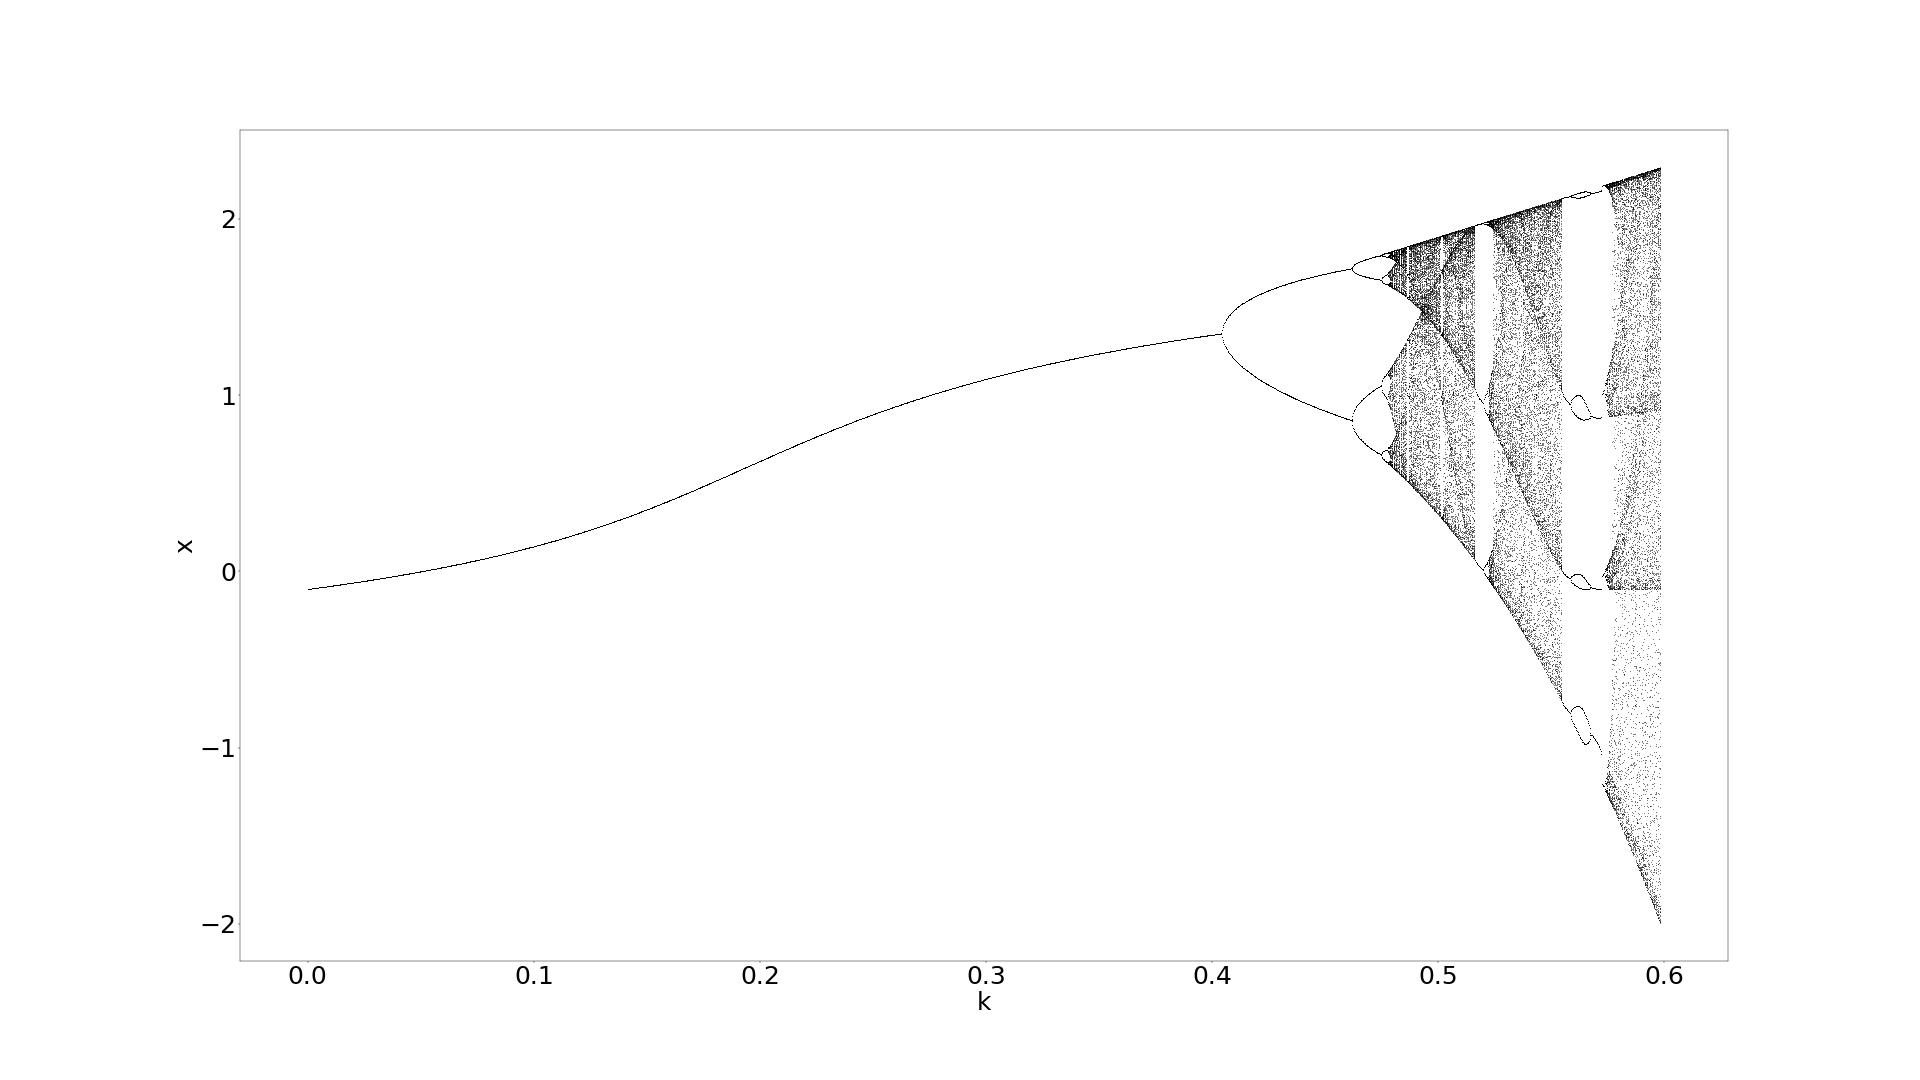
\includegraphics[width=0.6\linewidth]{LateX images/graphs/g1}
	\caption{ Διάγραμμα διακλάδωσης, για a=1, b=2 και q=-0.1}
	\label{f:g1}
\end{figure}



\begin{figure}[h!]
	\centering
	\caption{}
	\label{f:g2}
	\begin{subfigure}[b]{0.4\textwidth}
		\centering
		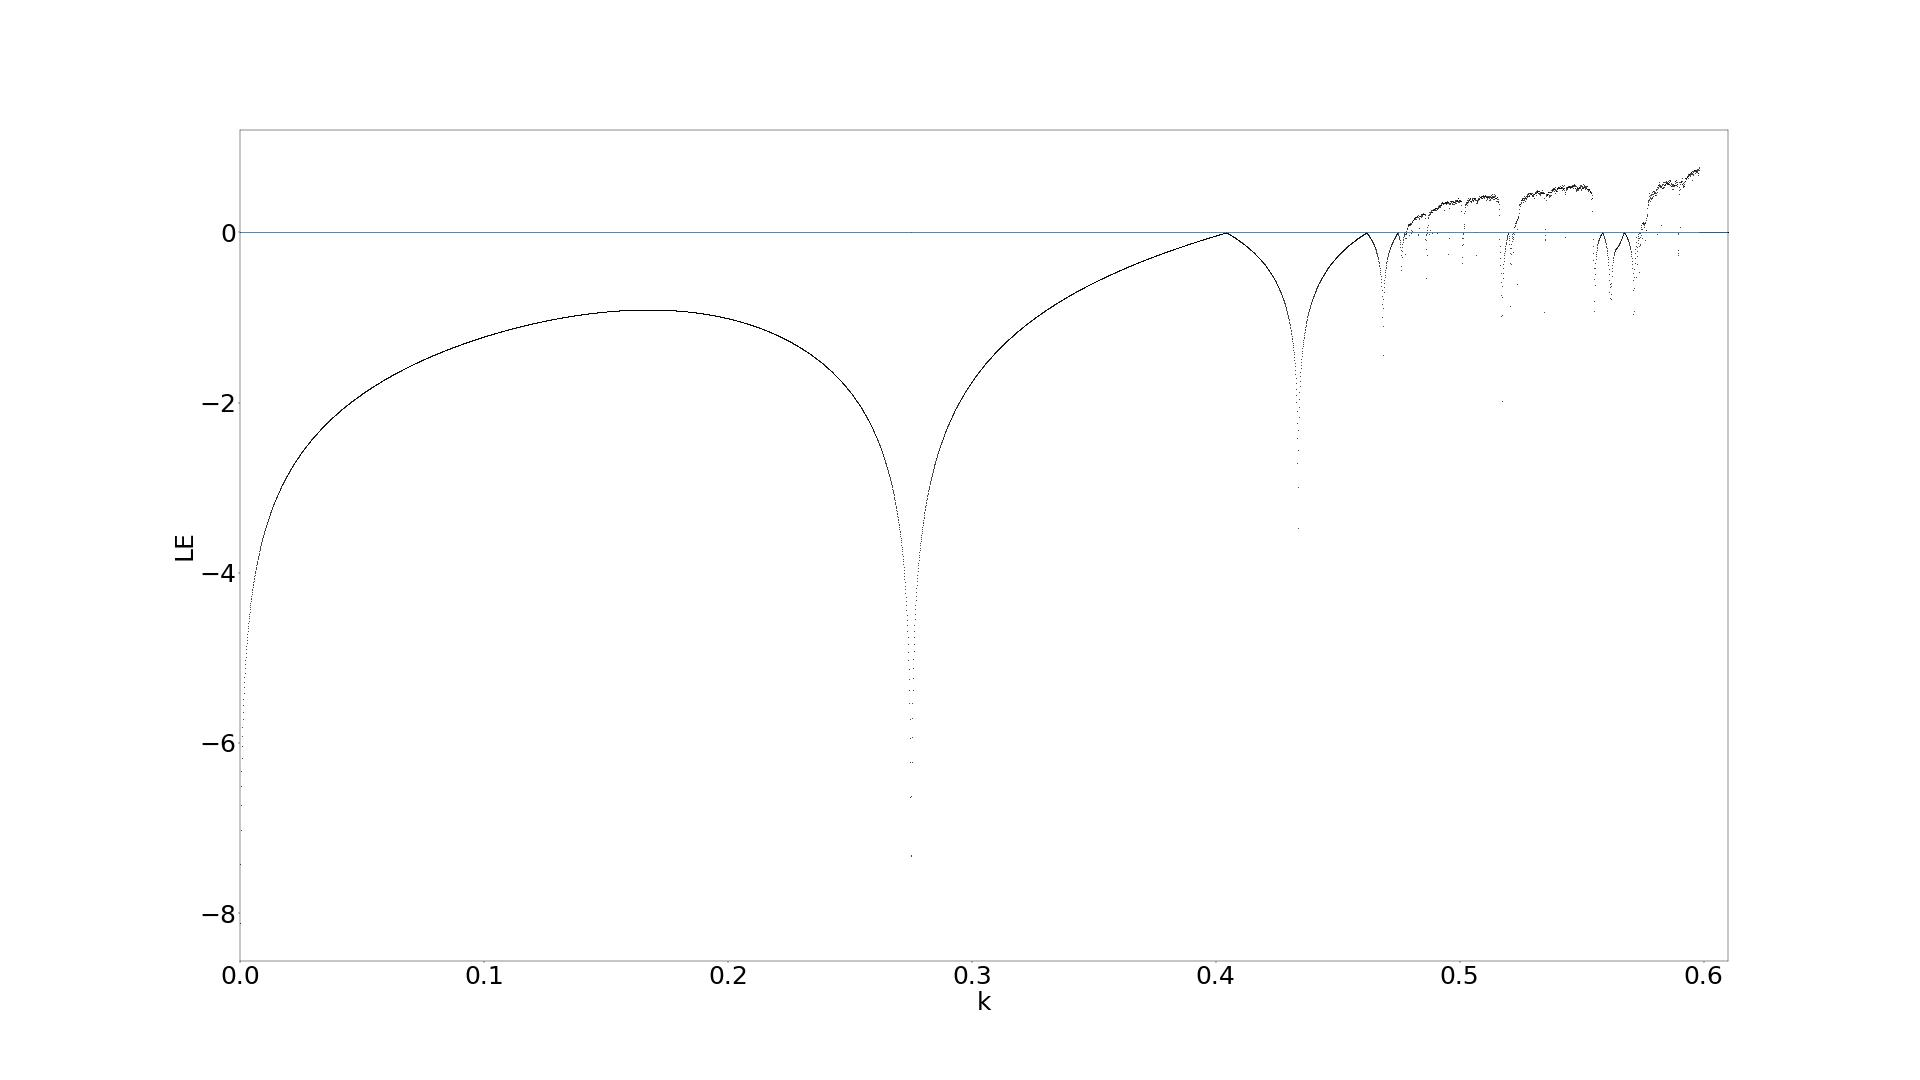
\includegraphics[width=\textwidth]{LateX images/graphs/g2}
		\caption{Διάγραμμα διακλάδωσης, για q=-0.112}
		\label{f:g3}
	\end{subfigure}
	\hfill
	\begin{subfigure}[b]{0.4\textwidth}
		\centering
		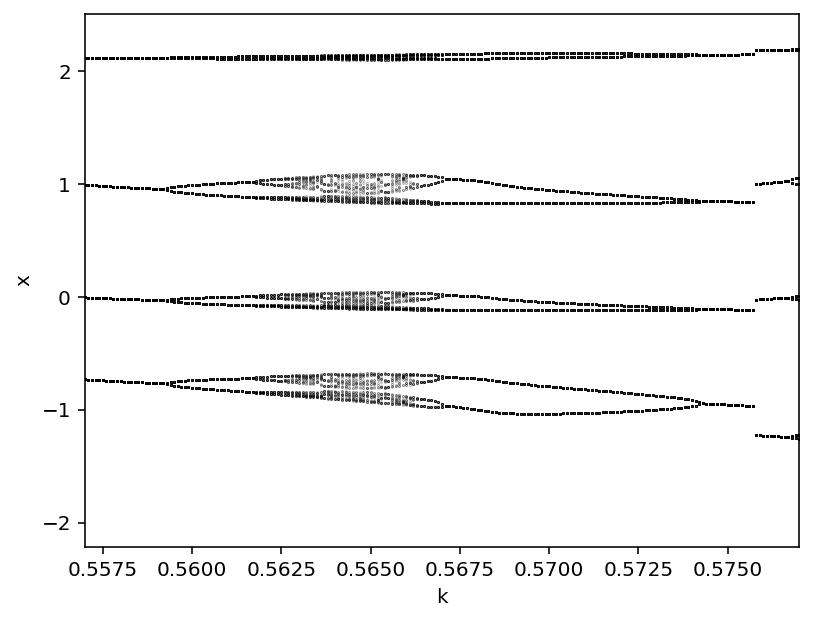
\includegraphics[width=\textwidth]{LateX images/graphs/g3}
		\caption{Διάγραμμα διακλάδωσης, για q=-0.114}
		\label{f:g4}
	\end{subfigure}
	\hfill
	\begin{subfigure}[b]{0.4\textwidth}
		\centering
		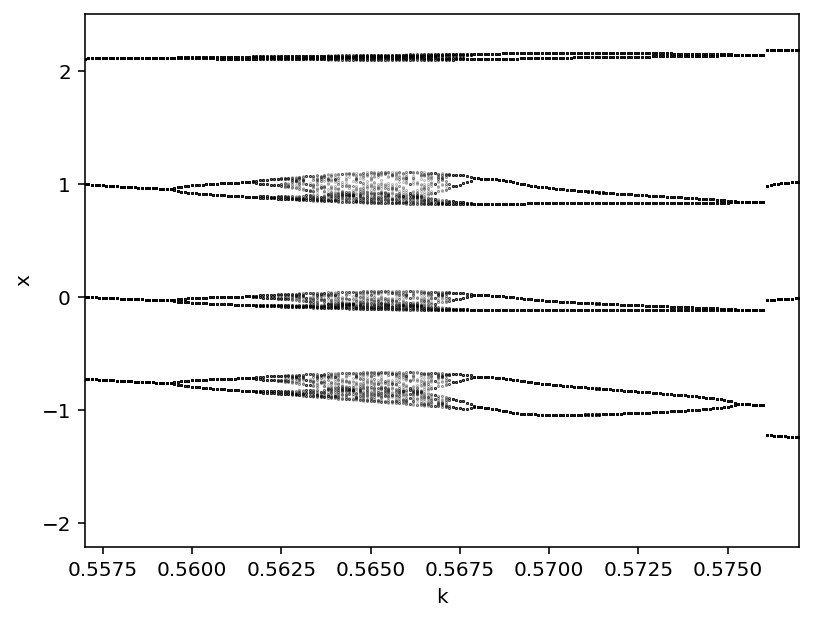
\includegraphics[width=\textwidth]{LateX images/graphs/g4}
		\caption{Διάγραμμα διακλάδωσης, για q=-0.116}
		\label{f:g5}
	\end{subfigure}
	\hfill
	\begin{subfigure}[b]{0.4\textwidth}
		\centering
		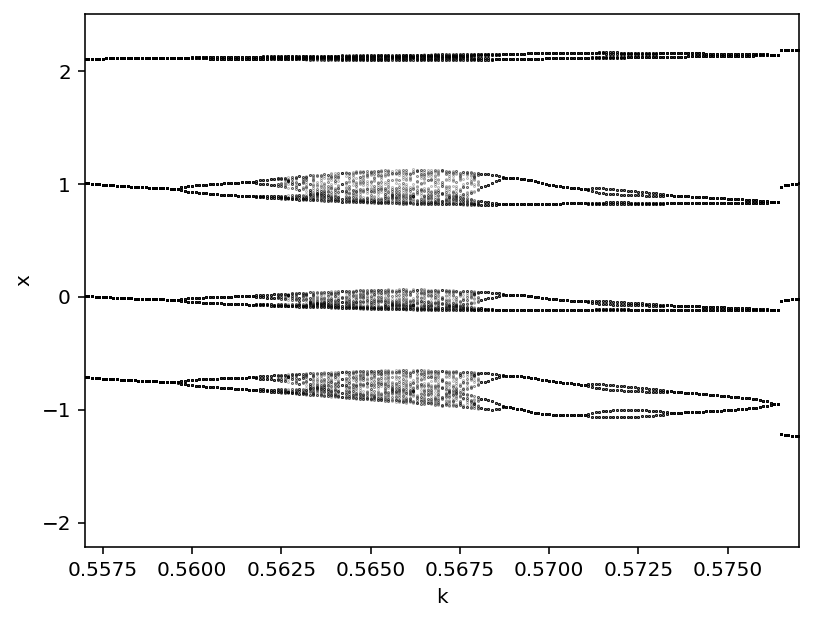
\includegraphics[width=\textwidth]{LateX images/graphs/g5}
		\caption{Διάγραμμα διακλάδωσης, για q=-0.118}
		\label{f:g6}
	\end{subfigure}
\end{figure}

\begin{figure}[h!]
	\centering
	\includegraphics[width=0.6\linewidth]{"LateX images/graphs/g6 "}
	\caption{Διάγραμμα του εκθέτη Lyapunov σε συνάρτηση με την παράμετρο k, για a=1, b=2 και q=-0.1.}
	\label{f:g7}
\end{figure}



\begin{figure}[h!]
	\centering
	\caption{Διαγράμματα της τιμής \(x_i\) με την τιμή \(x_{i+1}\) :}
	\begin{subfigure}[b]{0.25\textwidth}
		\centering
		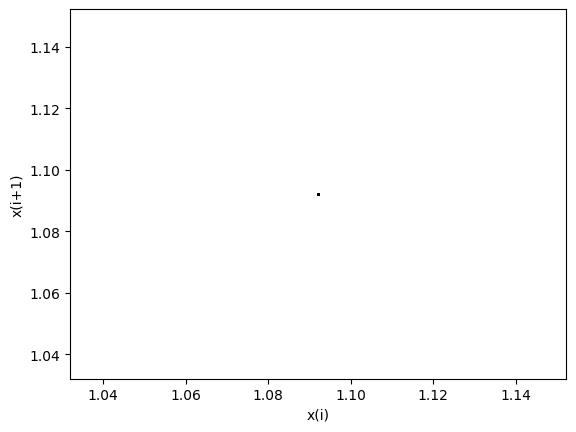
\includegraphics[width=\textwidth]{LateX images/graphs/k03}
		\caption{Για k=0.3}
		\label{f:k1}
	\end{subfigure}
	\hfill
	\begin{subfigure}[b]{0.25\textwidth}
		\centering
		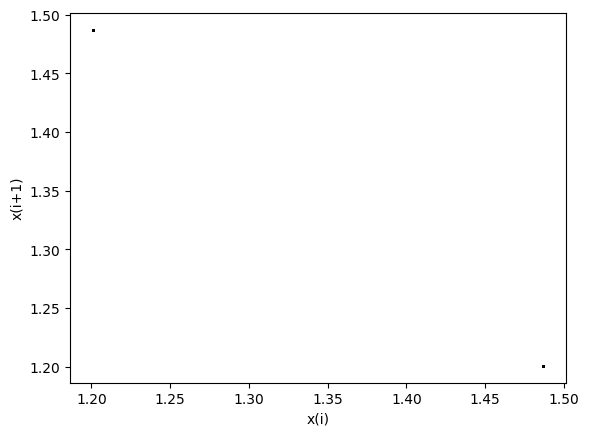
\includegraphics[width=\textwidth]{LateX images/graphs/k041}
		\caption{Για k=0.41}
		\label{f:k2}
	\end{subfigure}
	\hfill
	\begin{subfigure}[b]{0.25\textwidth}
		\centering
		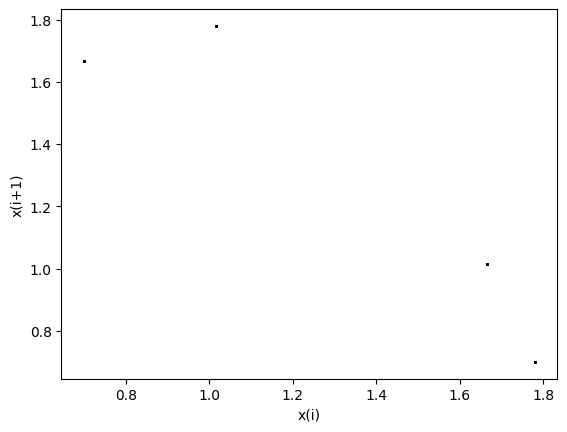
\includegraphics[width=\textwidth]{LateX images/graphs/k047}
		\caption{Για k=0.047}
		\label{f:k3}
	\end{subfigure}
	\begin{subfigure}[b]{0.25\textwidth}
		\centering
		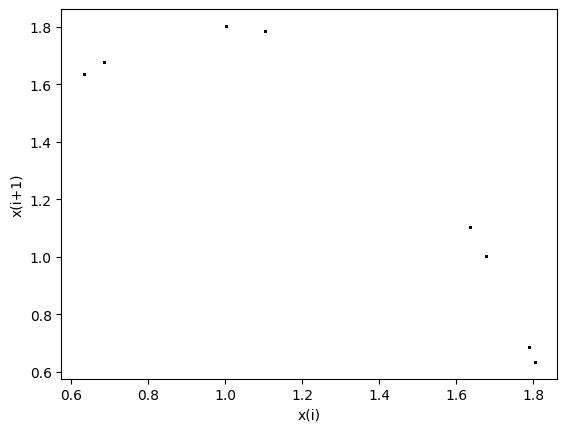
\includegraphics[width=\textwidth]{LateX images/graphs/k0476}
		\caption{Για k=0.476}
		\label{f:k4}
	\end{subfigure}
	\hfill
	\begin{subfigure}[b]{0.25\textwidth}
		\centering
		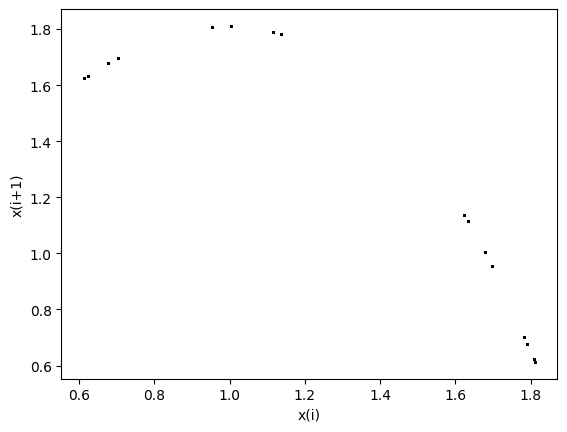
\includegraphics[width=\textwidth]{LateX images/graphs/k04778}
		\caption{Για k=0.4778}
		\label{f:k5}
	\end{subfigure}
	\hfill
	\begin{subfigure}[b]{0.25\textwidth}
		\centering
		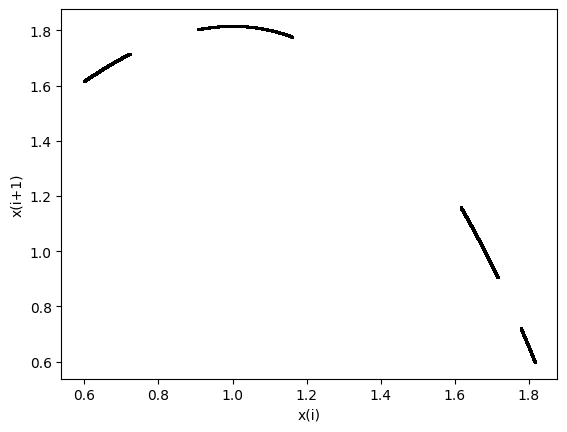
\includegraphics[width=\textwidth]{LateX images/graphs/k0479}
		\caption{Για k=0.479}
		\label{f:k6}
	\end{subfigure}
	\hfill
	\begin{subfigure}[b]{0.25\textwidth}
		\centering
		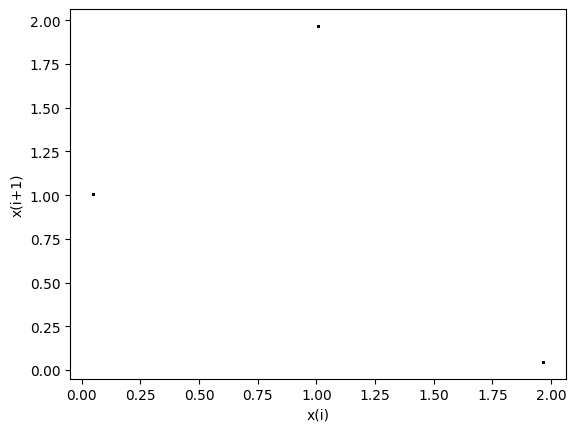
\includegraphics[width=\textwidth]{LateX images/graphs/k0517}
		\caption{Για k=0.517}
	\end{subfigure}
	\hfill
	\begin{subfigure}[b]{0.25\textwidth}
		\centering
		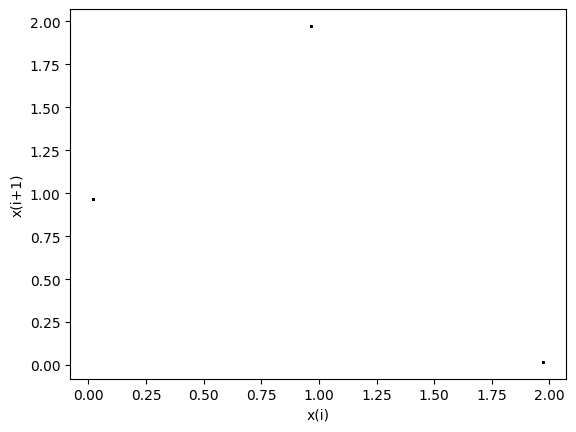
\includegraphics[width=\textwidth]{LateX images/graphs/k0519}
		\caption{Για k=0.519}
		\label{f:k7}
	\end{subfigure}
	\hfill
	\begin{subfigure}[b]{0.25\textwidth}
		\centering
		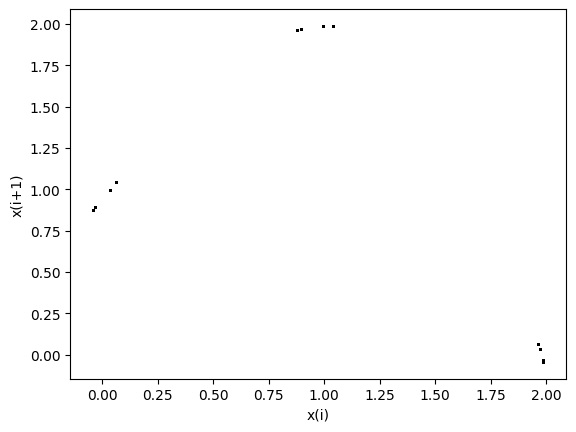
\includegraphics[width=\textwidth]{LateX images/graphs/k0522}
		\caption{Για k=0.522}
		\label{f:k8}
	\end{subfigure}
	\hfill
	\begin{subfigure}[b]{0.25\textwidth}
		\centering
		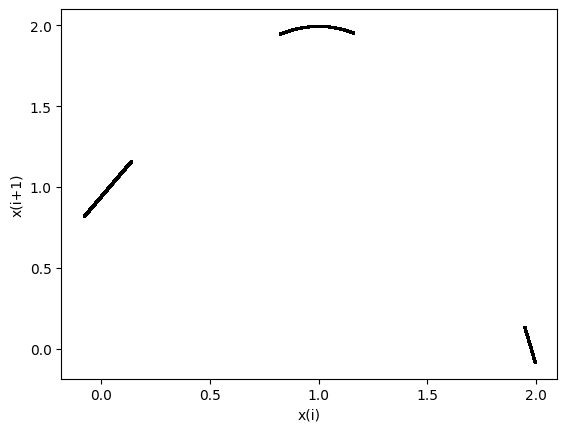
\includegraphics[width=\textwidth]{LateX images/graphs/k0524}
		\caption{Για k=0.524}
		\label{f:k9}
	\end{subfigure}
	\hfill
	\begin{subfigure}[b]{0.25\textwidth}
		\centering
		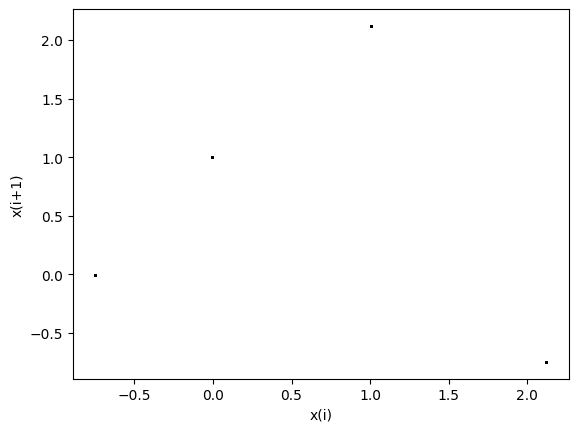
\includegraphics[width=\textwidth]{LateX images/graphs/k0555}
		\caption{Για k=0.555}
		\label{f:k10}
	\end{subfigure}
	\hfill
	\begin{subfigure}[b]{0.25\textwidth}
		\centering
		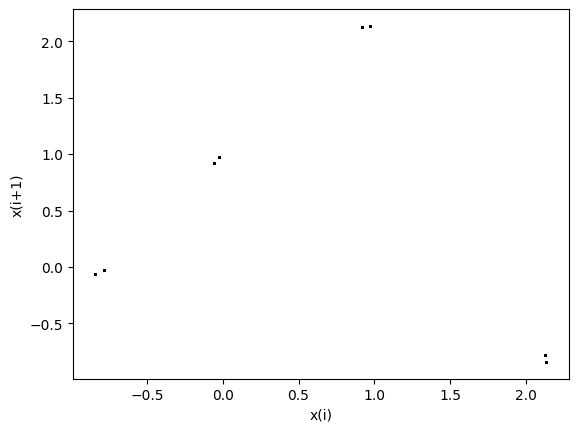
\includegraphics[width=\textwidth]{LateX images/graphs/k0559}
		\caption{Για k=0.559}
		\label{f:k11}
	\end{subfigure}
	\hfill
	\begin{subfigure}[b]{0.25\textwidth}
		\centering
		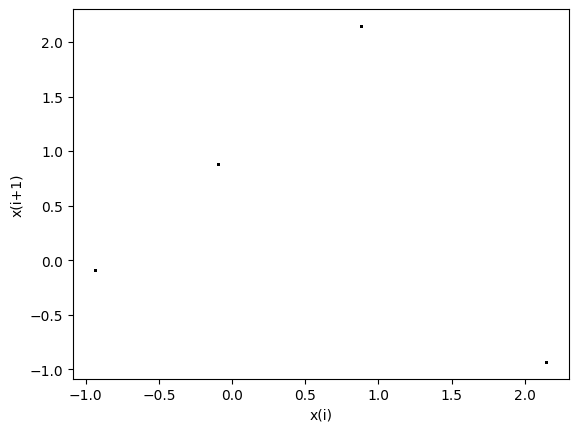
\includegraphics[width=\textwidth]{LateX images/graphs/k0568}
		\caption{Για k=0.568}
		\label{f:k12}
	\end{subfigure}
	\hfill
	\begin{subfigure}[b]{0.25\textwidth}
		\centering
		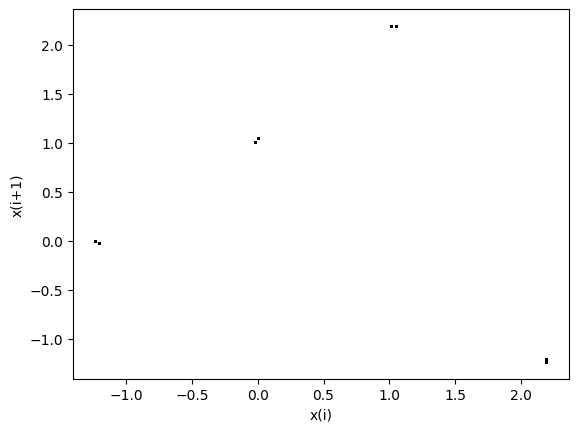
\includegraphics[width=\textwidth]{LateX images/graphs/k05735}
		\caption{Για k=0.5735}
		\label{f:k13}
	\end{subfigure}
	\hfill
	\begin{subfigure}[b]{0.25\textwidth}
		\centering
		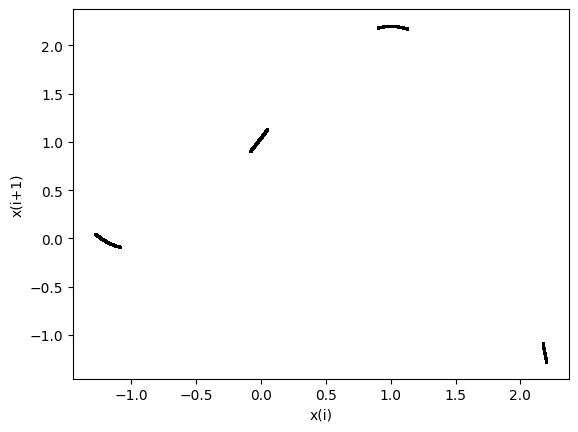
\includegraphics[width=\textwidth]{LateX images/graphs/k0575}
		\caption{Για k=0.575}
		\label{f:k14}
	\end{subfigure}

\end{figure}

 \clearpage
\subsection{Για q=-0.3}

Στο σχήμα \ref{f:g8} παρατίθεται το διάγραμμα διακλάδωσης του συστήματος \ref{f:x1}, ως προς την παράμετρο k, για a=1, b=2 και q =- 0.3. Για αυτές τις τιμές των παραμέτρων το σύστημα ξεκινάει από περίοδο-1 για k = 0.3 , ενώ για  k = 0.44 εμφανίζει τον πρώτο διπλασιασμό της περιόδου. Τον δεύτερο διπλασιασμό τον εμφανίζει για k=0.5 (περίοδος-4) ,τον τρίτο για k=0.511(περίοδος-8).Στην συνέχεια για k>0.5165 το σύστημα εισέρχεται στο χάος , μέχρι να εξέλθει  για k=0.551(περίοδος-3) και να ξανά εισέλθει σε χάος μετά από δύο διπλασιασμούς k=0.555(περίοδος-6) και k=0.556(περίοδος-12) για k>0.5573. To φαινόμενο αυτό είναι γνωστό ως συνοριακή κρίση .Εξέρχεται για τελευταία φορά από το χάος για k=0.583 (περίοδος-4) και μετά απο ένα διπλασιασμό  για k=0.5846(Περίόδος-7) είσέρχεται για τελευταία φορά στο χάος για k=0.5851.
Επομένως και σε αυτή την περίπτωση το σύστημα εισέρχεται στο χάος με διπλασιασμό της περιόδου. 
Επιπλέον, στο σχήμα \ref{f:g9} παρατίθεται το διάγραμμα των εκθετών Lyapunov για τιμές του k στο ίδιο διάστημα τιμών [0, 0.63].  Στο διάστημα τιμών   0<k<0.511 , στο 0.551<k<0.556, και στο 0.583<k<0.5846 παρατηρούμε ότι ο εκθέτης Lyapunov είναι συνεχώς αρνητικός, γεγονός που επιβεβαιώνει την περιοδική συμπεριφορά του συστήματος. Ενώ στα υπόλοιπα διαστήματα ο θετικός εκθέτης Lyapunov υποστηρίζει την χαοτική του συμπεριφορά, όπως έγινε φανερό και από το διάγραμμα διακλάδωσης.
Τέλος, στον Πίνακα \ref{tab:abc1} παρατίθενται ενδεικτικές τιμές της παραμέτρου k και η συμπεριφορά που παρουσιάζει το σύστημα για αυτές, σύμφωνα με το διάγραμμα διακλάδωσης, καθώς και τα αντίστοιχα σχήματα των διαγραμμάτων της τιμής \(x_i\) σε συνάρτηση με την τιμή \(x_{i+1}\). Από τα παραγόμενα σχήματα προκύπτει αριθμός σημείων αντίστοιχος με την περίοδο του συστήματος.
\begin{table}[h!]
	\centering
	\begin{tabular}{l | l | l}
		Παράμετρος k & Συμπεριφορά & Σχήμα\\
		\hline
		0.3 &  Περίοδος-1 & \ref{f:k1}\\
		0.44& Περίοδος-2 & \ref{f:k2}\\
		0.5& Περίοδος-4 & \ref{f:k2}\\
		0.511 &  Περίοδος-8 & \ref{f:k3}\\
		0.5165 & Χάος & \ref{f:k5}\\
		0.551 & Περίοδος-3 & \ref{f:k6})\\
		0.555 & Περίοδος-6 & \ref{f:k7}\\
		0.556 & Περίοδος-12 & \ref{f:k8}\\
		0.5573 & Χάος & \ref{f:k9}\\
		0.583& Περίοδος-4 & \ref{f:k10}\\
		0.5846 & Περίοδος-7 & \ref{f:k11}\\
		0.5851 & Χάος & \ref{f:k14}\\
	\end{tabular}
	\caption{ Συμπεριφορά του υπό μελέτη συστήματος για διάφορες τιμές του k,για a=1, b=2 και q=-0.3}
	\label{tab:abc1}
\end{table}

\begin{figure}[h!]
	\centering
	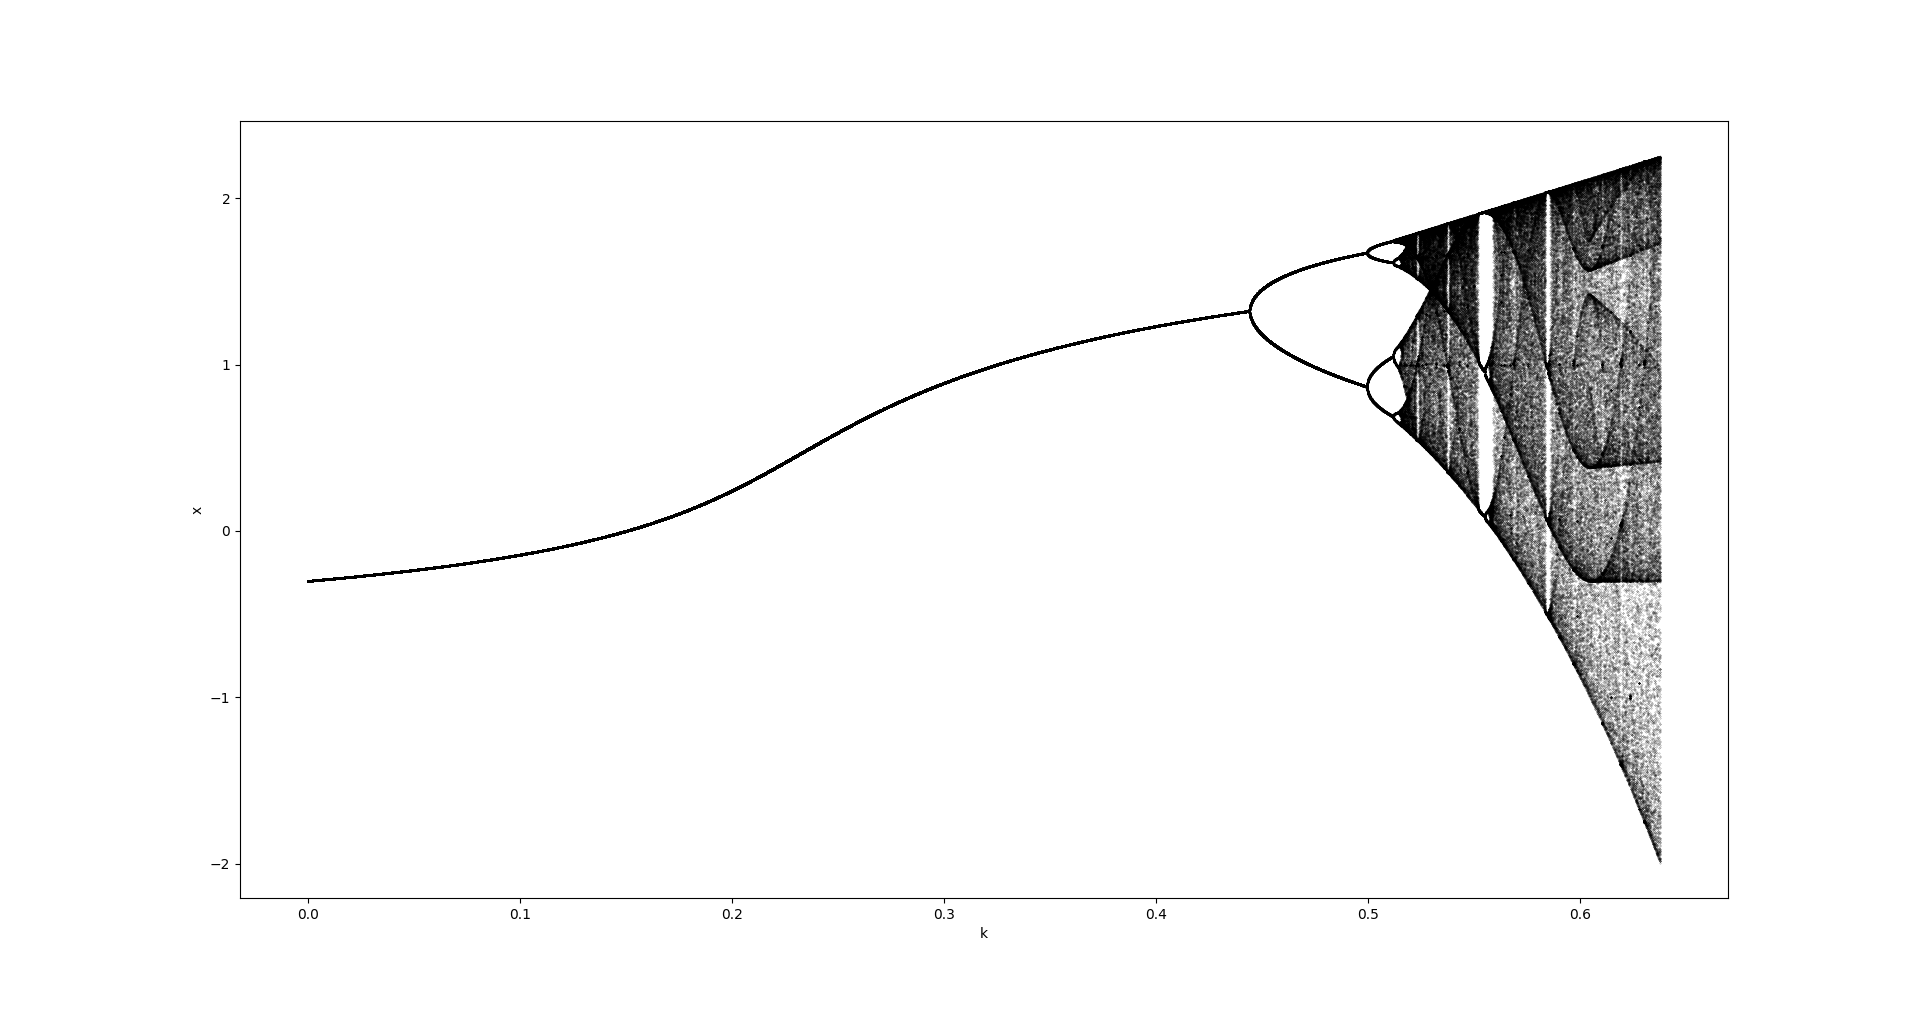
\includegraphics[width=0.6\linewidth]{LateX images/graphs q03/g1}
	\caption{ Διάγραμμα διακλάδωσης, για a=1, b=2 και q=-0.3}
	\label{f:g8}
\end{figure}

\begin{figure}[h!]
	\centering
	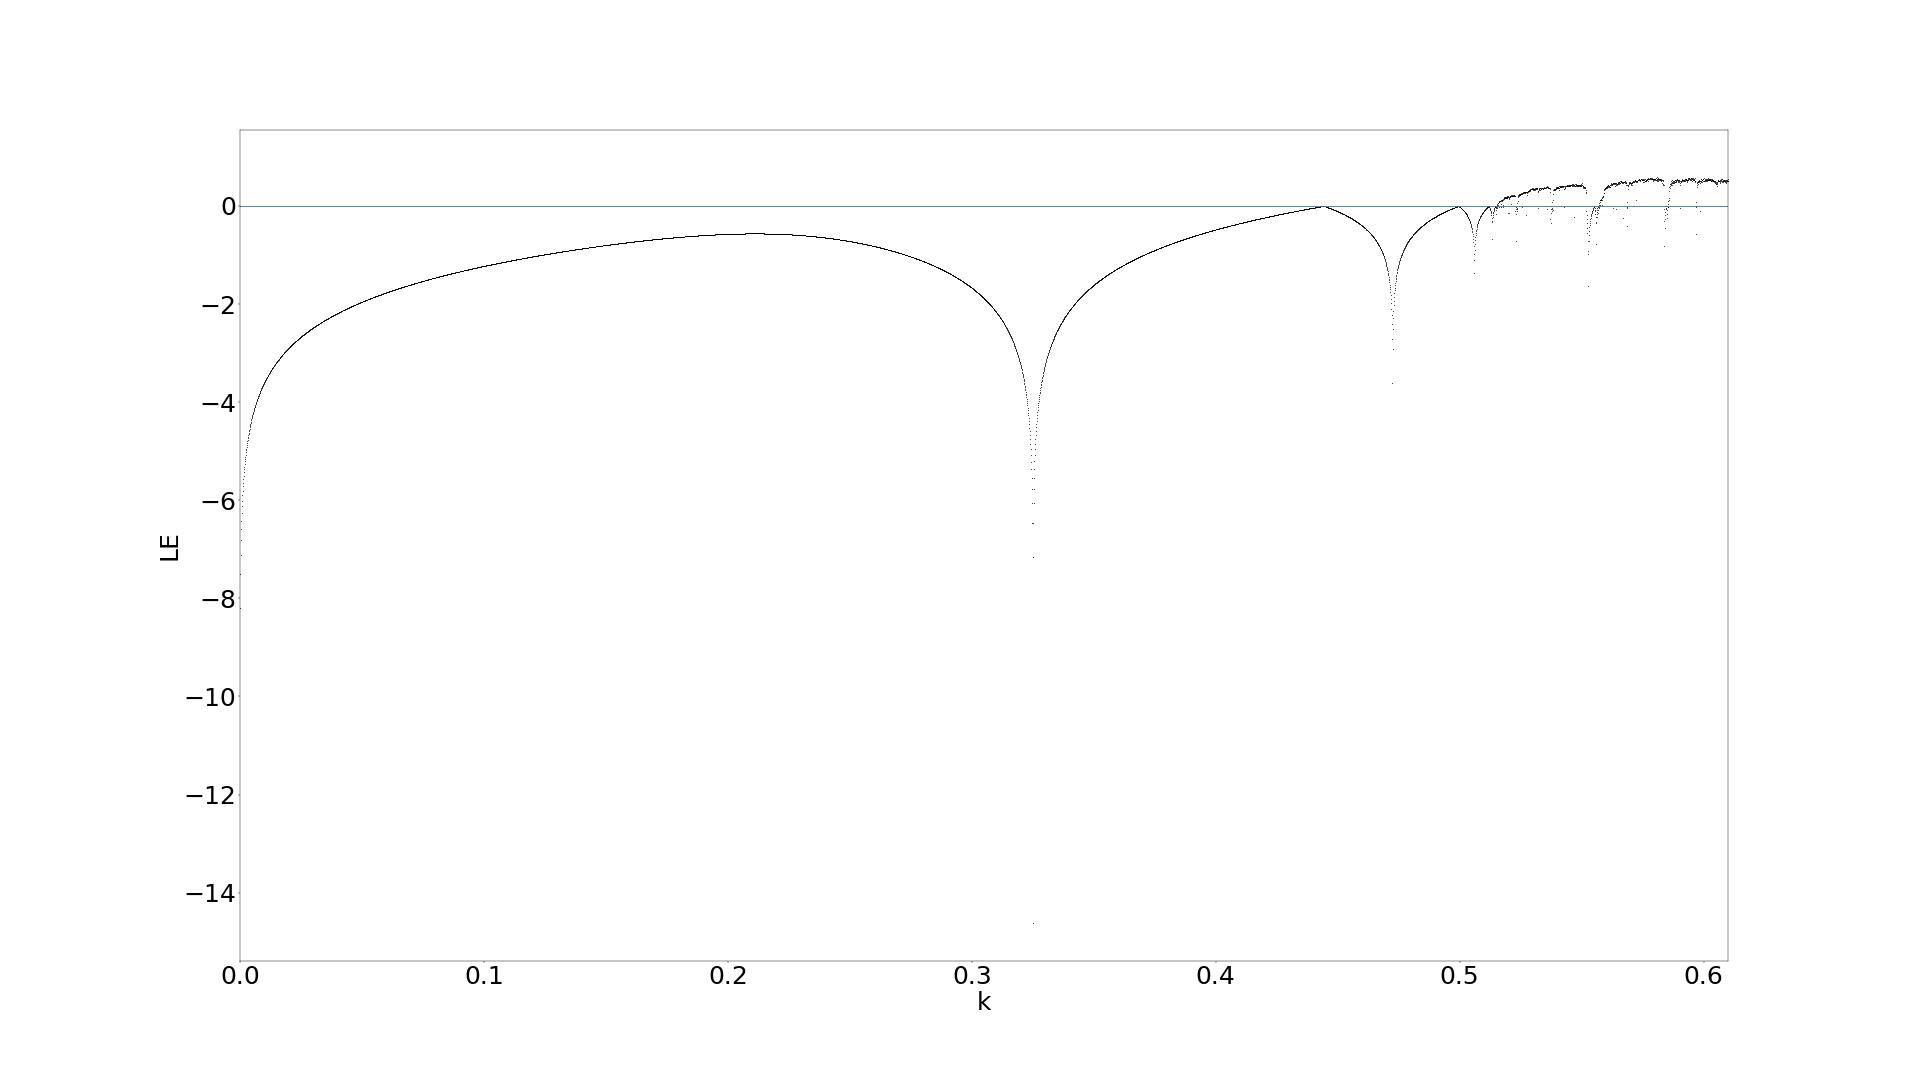
\includegraphics[width=0.6\linewidth]{LateX images/graphs q03/g2}
	\caption{ Διάγραμμα του εκθέτη Lyapunov σε συνάρτηση με την παράμετρο k, για a=1, b=2 και q=-0.3}
	\label{f:g9}
\end{figure}

\begin{figure}[h!]
	\centering
	\caption{Διαγράμματα της τιμής \(x_i\) με την τιμή \(x_{i+1}\) :}
	\begin{subfigure}[b]{0.25\textwidth}
		\centering
		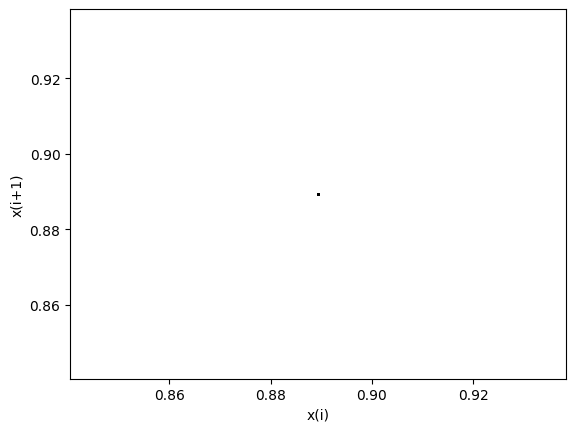
\includegraphics[width=\textwidth]{LateX images/graphs q03/g3}
		\caption{Για k=0.3}
		\label{f:k15}
	\end{subfigure}
	\hfill
	\begin{subfigure}[b]{0.25\textwidth}
		\centering
		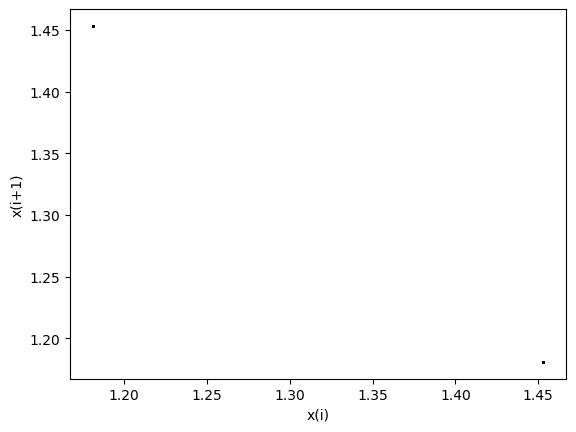
\includegraphics[width=\textwidth]{LateX images/graphs q03/g4}
		\caption{Για k=0.44}
		\label{f:k16}
	\end{subfigure}
	\hfill
	\begin{subfigure}[b]{0.25\textwidth}
		\centering
		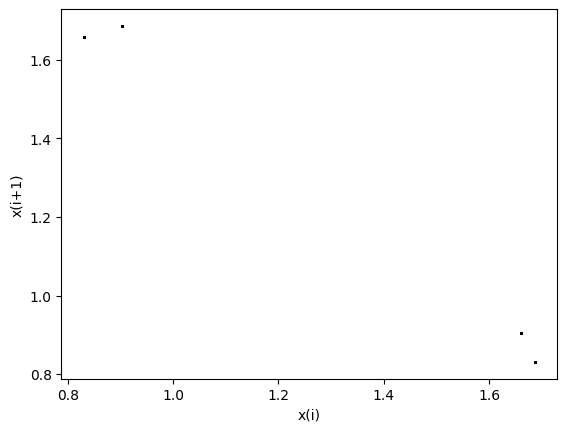
\includegraphics[width=\textwidth]{LateX images/graphs q03/g5}
		\caption{Για k=0.5}
		\label{f:k17}
	\end{subfigure}
	\hfill
	\begin{subfigure}[b]{0.25\textwidth}
		\centering
		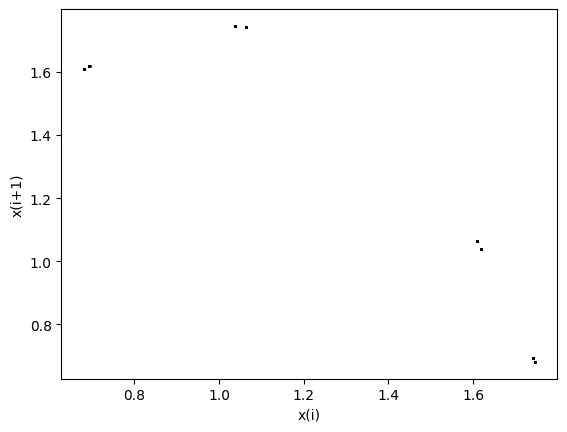
\includegraphics[width=\textwidth]{LateX images/graphs q03/g6}
		\caption{Για k=0.511}
		\label{f:k18}
	\end{subfigure}
	\hfill
	\begin{subfigure}[b]{0.25\textwidth}
		\centering
		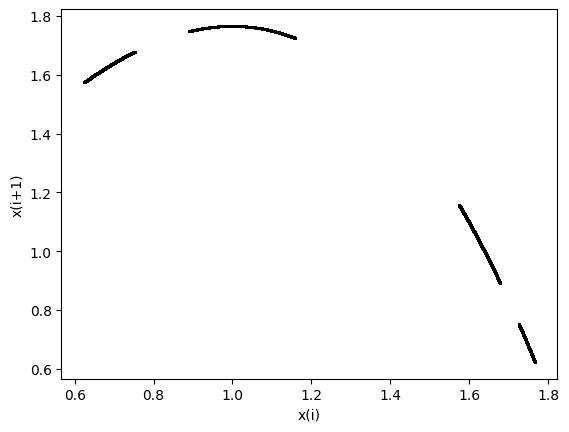
\includegraphics[width=\textwidth]{LateX images/graphs q03/g67}
		\caption{Για k=0.5165}
		\label{f:k19}
	\end{subfigure}
	\hfill
	\begin{subfigure}[b]{0.25\textwidth}
		\centering
		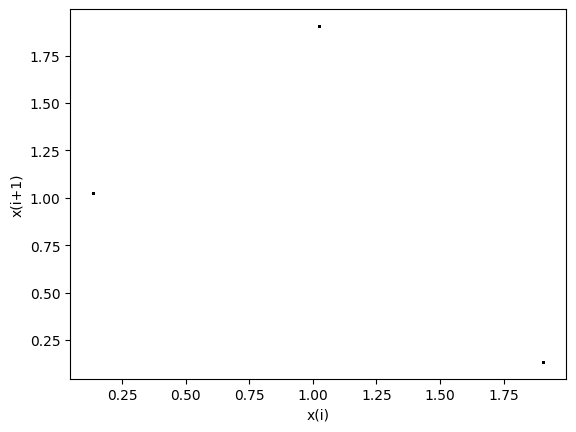
\includegraphics[width=\textwidth]{LateX images/graphs q03/g8}
		\caption{Για k=0.551}
		\label{f:k20}
	\end{subfigure}
	\hfill
	\begin{subfigure}[b]{0.25\textwidth}
		\centering
		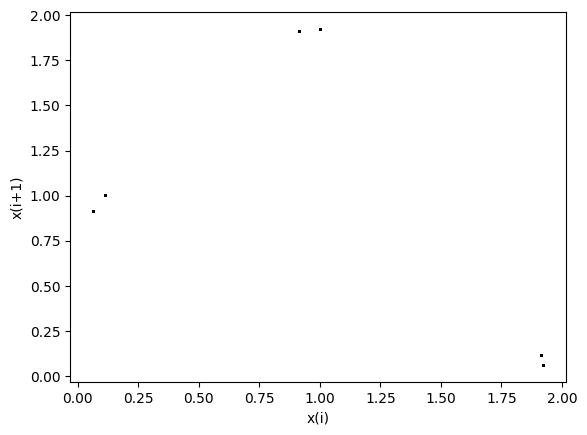
\includegraphics[width=\textwidth]{LateX images/graphs q03/g9}
		\caption{Για k=0.555}
		\label{f:k21}
	\end{subfigure}
	\hfill
	\begin{subfigure}[b]{0.25\textwidth}
		\centering
		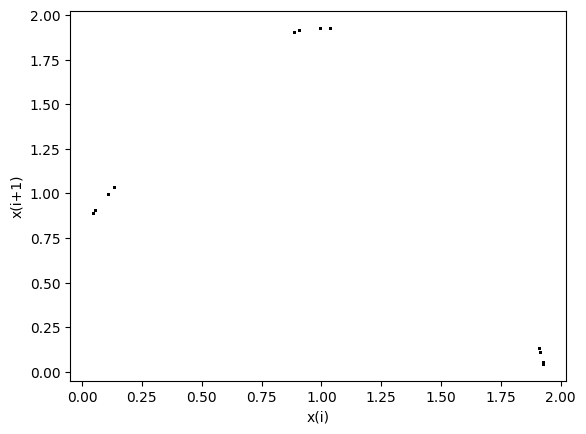
\includegraphics[width=\textwidth]{LateX images/graphs q03/g10}
		\caption{Για k=0.556}
		\label{f:k22}
	\end{subfigure}
	\hfill
	\begin{subfigure}[b]{0.25\textwidth}
		\centering
		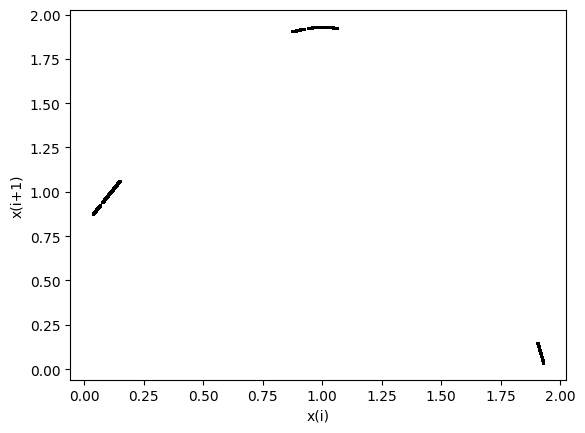
\includegraphics[width=\textwidth]{LateX images/graphs q03/g11}
		\caption{Για k=0.5573}
		\label{f:k23}
	\end{subfigure}
	\hfill
	\begin{subfigure}[b]{0.25\textwidth}
		\centering
		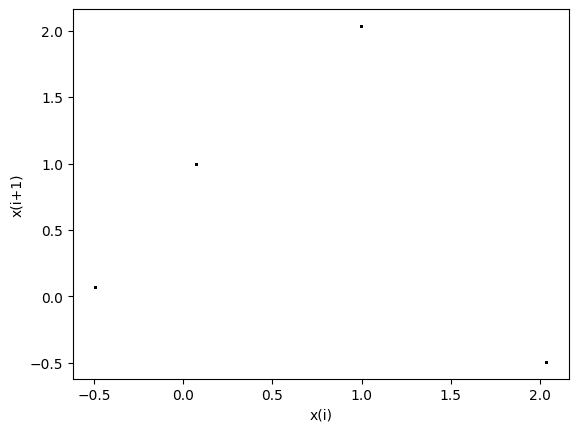
\includegraphics[width=\textwidth]{LateX images/graphs q03/g12}
		\caption{Για k=0.583}
		\label{f:k24}
	\end{subfigure}
	\hfill
	\begin{subfigure}[b]{0.25\textwidth}
		\centering
		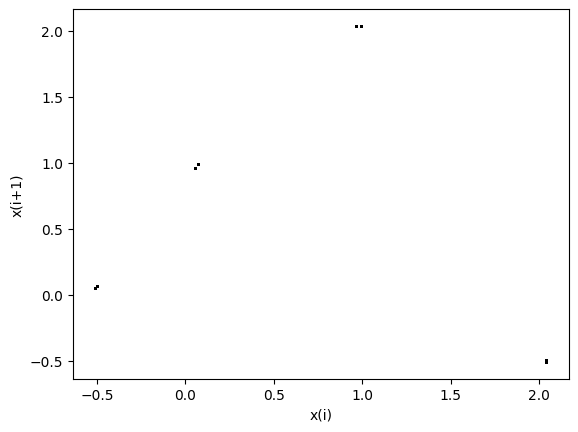
\includegraphics[width=\textwidth]{LateX images/graphs q03/g13}
		\caption{Για k=0.5846}
		\label{f:k25}
	\end{subfigure}
	\hfill
	\begin{subfigure}[b]{0.25\textwidth}
		\centering
		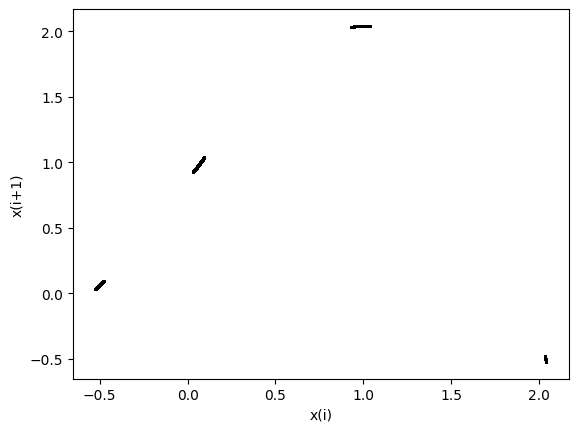
\includegraphics[width=\textwidth]{LateX images/graphs q03/g14}
		\caption{Για k=0.5851}
		\label{f:k26}
	\end{subfigure}
	
\end{figure}

\clearpage

\subsection{Για q=-0.5}

Στο σχήμα \ref{f:g10} παρατίθεται το διάγραμμα διακλάδωσης του συστήματος \ref{f:x1}, ως προς την παράμετρο k, για a=1, b=2 και q =- 0.5. Για αυτές τις τιμές των παραμέτρων το σύστημα ξεκινάει από περίοδο-1 για k = 0.3 , ενώ για  k = 0.48 εμφανίζει τον πρώτο διπλασιασμό της περιόδου. Τον δεύτερο διπλασιασμό τον εμφανίζει για k=0.53 (περίοδος-4) ,τον τρίτο για k=0.55 (περίοδος-8) και τον τέταρτο για k=0.5531 (περόδος-15).Στην συνέχεια για k>0.5534 το σύστημα εισέρχεται στο χάος , μέχρι να εξέλθει  για k=0.59(περίοδος-3) και να ξανά εισέλθει σε χάος μετά από δύο διπλασιασμούς k=0.59377 (περίοδος-6) ,για k>0.594.
Επομένως και σε αυτή την περίπτωση το σύστημα εισέρχεται στο χάος με διπλασιασμό της περιόδου. 
Επιπλέον, στο σχήμα \ref{f:g11} παρατίθεται το διάγραμμα των εκθετών Lyapunov για τιμές του k στο ίδιο διάστημα τιμών [0, 0.67].  Στο διάστημα τιμών   0<k<0.511 , στο 0.551<k<0.556, και στο 0.583<k<0.5846 παρατηρούμε ότι ο εκθέτης Lyapunov είναι συνεχώς αρνητικός, γεγονός που επιβεβαιώνει την περιοδική συμπεριφορά του συστήματος. Ενώ στα υπόλοιπα διαστήματα ο θετικός εκθέτης Lyapunov υποστηρίζει την χαοτική του συμπεριφορά, όπως έγινε φανερό και από το διάγραμμα διακλάδωσης.
Τέλος, στον Πίνακα \ref{tab:abc2} παρατίθενται ενδεικτικές τιμές της παραμέτρου k και η συμπεριφορά που παρουσιάζει το σύστημα για αυτές, σύμφωνα με το διάγραμμα διακλάδωσης, καθώς και τα αντίστοιχα σχήματα των διαγραμμάτων της τιμής \(x_i\) σε συνάρτηση με την τιμή \(x_{i+1}\). Από τα παραγόμενα σχήματα προκύπτει αριθμός σημείων αντίστοιχος με την περίοδο του συστήματος.

\begin{table}[h!]
	\centering
	\begin{tabular}{l | l | l}
		Παράμετρος k & Συμπεριφορά & Σχήμα\\
		\hline
		0.3 &  Περίοδος-1 & \ref{f:k1}\\
		0.48& Περίοδος-2 & \ref{f:k2}\\
		0.53& Περίοδος-4 & \ref{f:k2}\\
		0.55 &  Περίοδος-8 & \ref{f:k3}\\
		0.5531 & Περίοδος-15 & \ \\
		0.5534 & Χάος & \ref{f:k5}\\
		0.59 & Περίοδος-3 & \ref{f:k6})\\
		0.593 & Περίοδος-6 & \ref{f:k7}\\
		0.594 & Χάος & \ref{f:k9}\\
	\end{tabular}
	\caption{ Συμπεριφορά του υπό μελέτη συστήματος για διάφορες τιμές του k,για a=1, b=2 και q=-0.5}
	\label{tab:abc2}
\end{table}

\begin{figure}[h!]
	\centering
	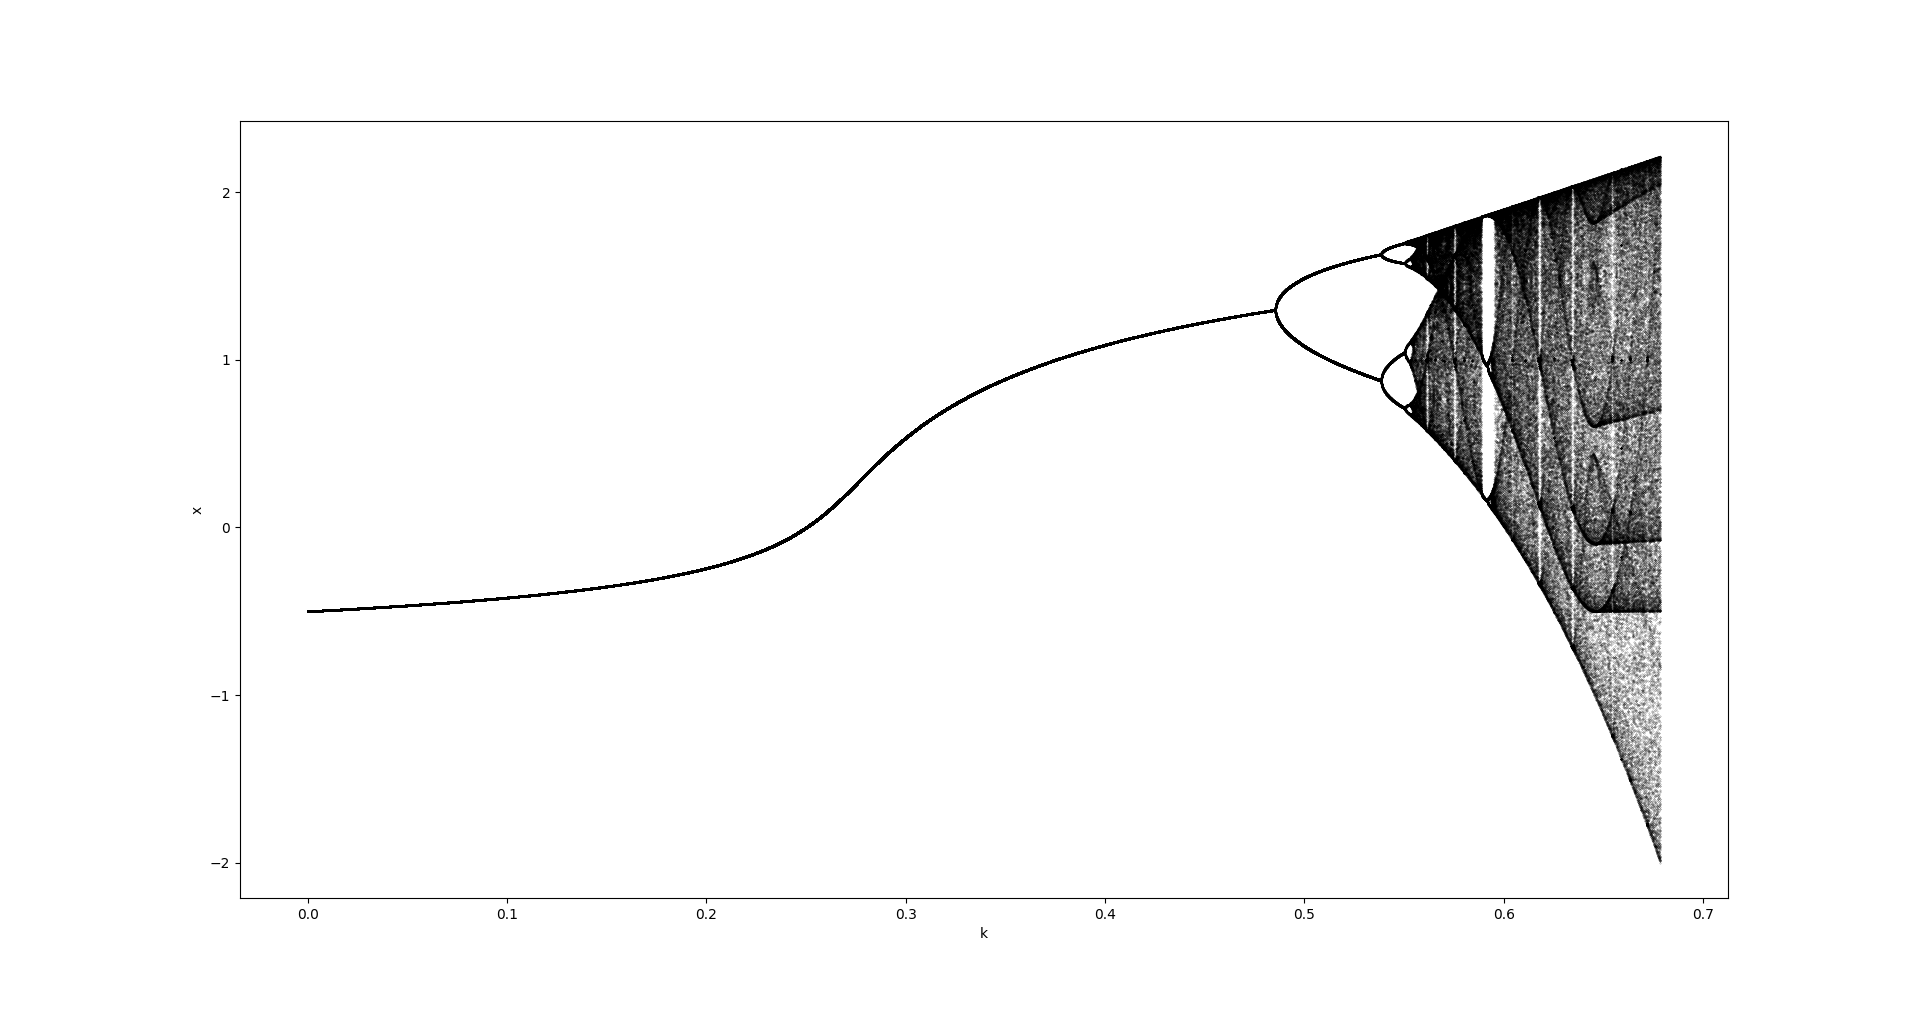
\includegraphics[width=0.6\linewidth]{LateX images/graphs q05/g1}
	\caption{ Διάγραμμα διακλάδωσης, για a=1, b=2 και q=-0.5}
	\label{f:g10}
\end{figure}

\begin{figure}[h!]
	\centering
	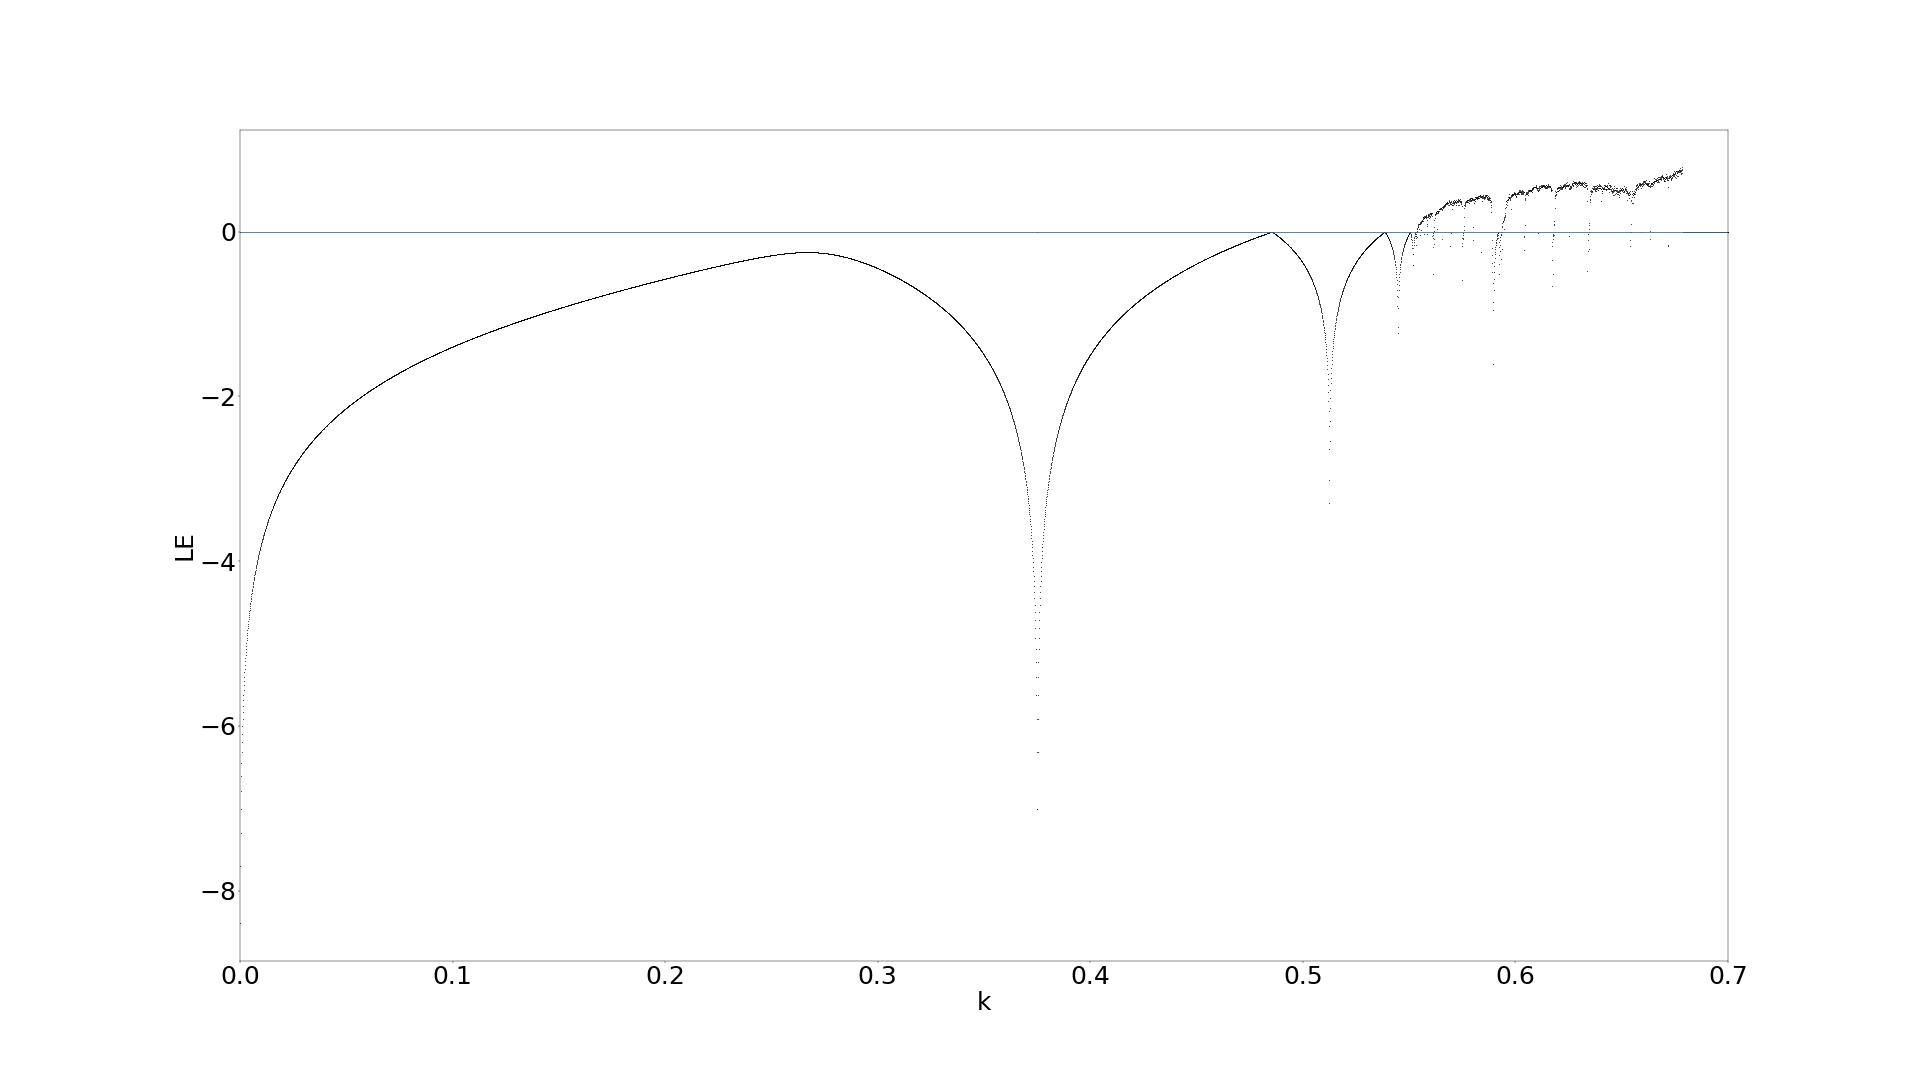
\includegraphics[width=0.6\linewidth]{LateX images/graphs q05/g2}
	\caption{ Διάγραμμα του εκθέτη Lyapunov σε συνάρτηση με την παράμετρο k, για a=1, b=2 και q=-0.5}
	\label{f:g11}
\end{figure}

\begin{figure}[h!]
	\centering
	\caption{Διαγράμματα της τιμής \(x_i\) με την τιμή \(x_{i+1}\) :}
	\begin{subfigure}[b]{0.25\textwidth}
		\centering
		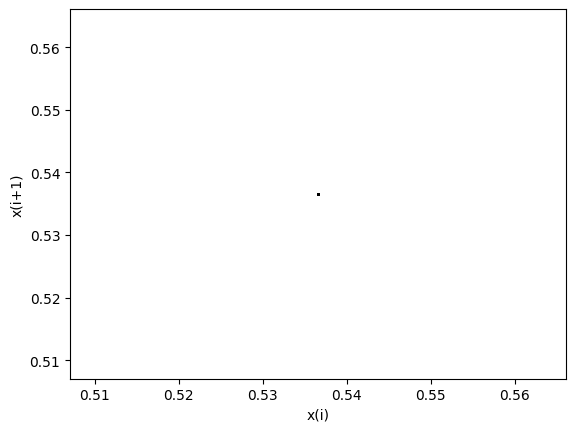
\includegraphics[width=\textwidth]{LateX images/graphs q05/g3}
		\caption{Για k=0.3}
		\label{f:k27}
	\end{subfigure}
	\hfill
	\begin{subfigure}[b]{0.25\textwidth}
		\centering
		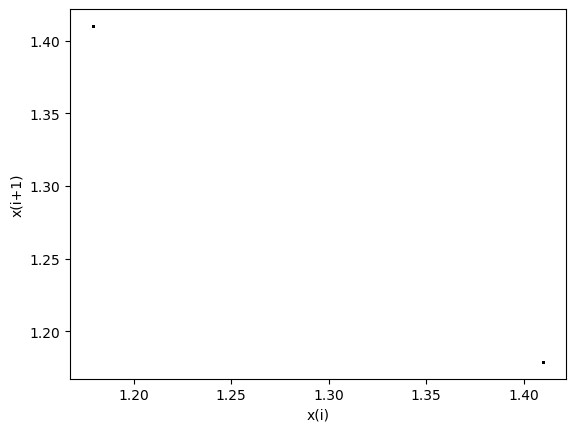
\includegraphics[width=\textwidth]{LateX images/graphs q05/g4}
		\caption{Για k=0.48}
		\label{f:k28}
	\end{subfigure}
	\hfill
	\begin{subfigure}[b]{0.25\textwidth}
		\centering
		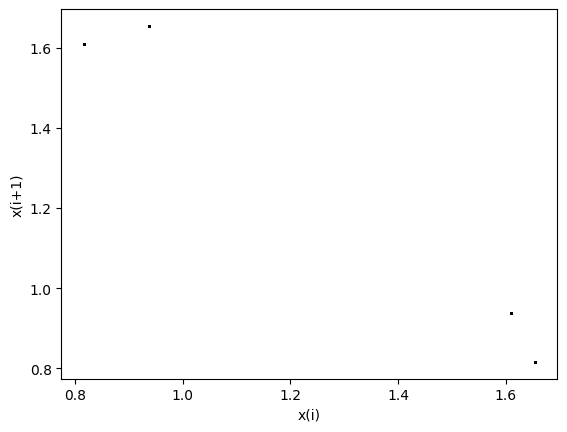
\includegraphics[width=\textwidth]{LateX images/graphs q05/g5}
		\caption{Για k=0.53}
		\label{f:k29}
	\end{subfigure}
	\begin{subfigure}[b]{0.25\textwidth}
		\centering
		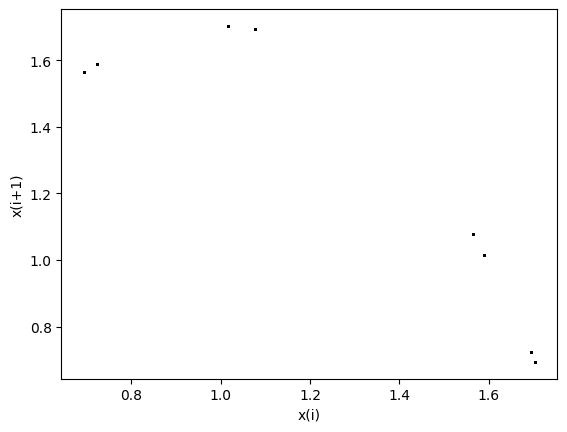
\includegraphics[width=\textwidth]{LateX images/graphs q05/g6}
		\caption{Για k=0.55}
		\label{f:k30}
	\end{subfigure}
	\hfill
	\begin{subfigure}[b]{0.25\textwidth}
		\centering
		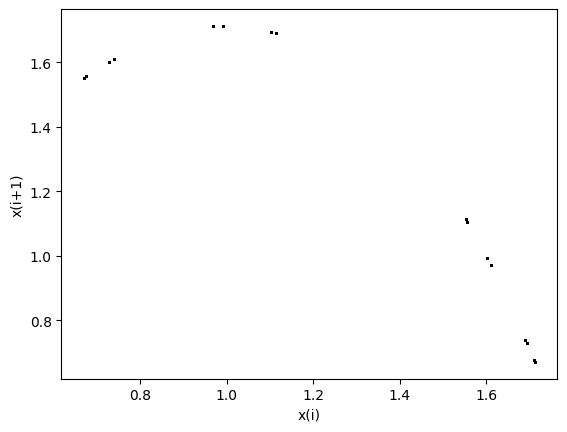
\includegraphics[width=\textwidth]{LateX images/graphs q05/g7}
		\caption{Για k=0.5531}
		\label{f:k31}
	\end{subfigure}
	\hfill
	\begin{subfigure}[b]{0.25\textwidth}
		\centering
		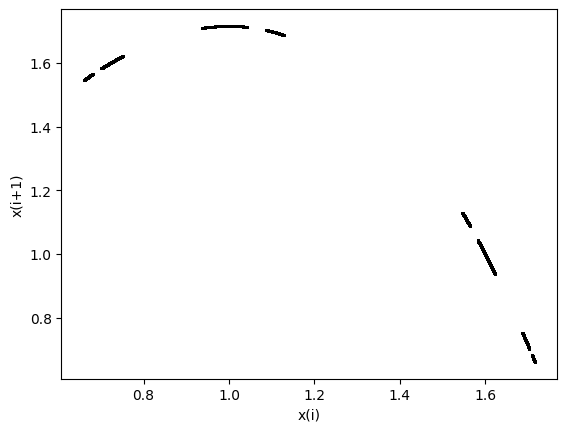
\includegraphics[width=\textwidth]{LateX images/graphs q05/g8}
		\caption{Για k=0.5534}
		\label{f:k32}
	\end{subfigure}
	\hfill
	\begin{subfigure}[b]{0.25\textwidth}
		\centering
		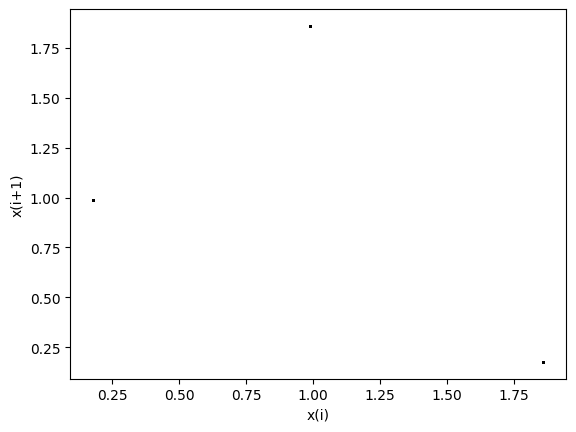
\includegraphics[width=\textwidth]{LateX images/graphs q05/g9}
		\caption{Για k=0.58}
		\label{f:k33}
	\end{subfigure}
	\hfill
	\begin{subfigure}[b]{0.25\textwidth}
		\centering
		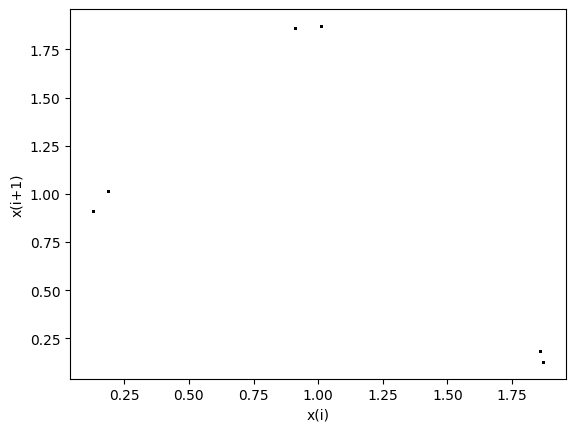
\includegraphics[width=\textwidth]{LateX images/graphs q05/g10}
		\caption{Για k=0.591}
		\label{f:k35}
	\end{subfigure}
	\hfill
	\begin{subfigure}[b]{0.25\textwidth}
		\centering
		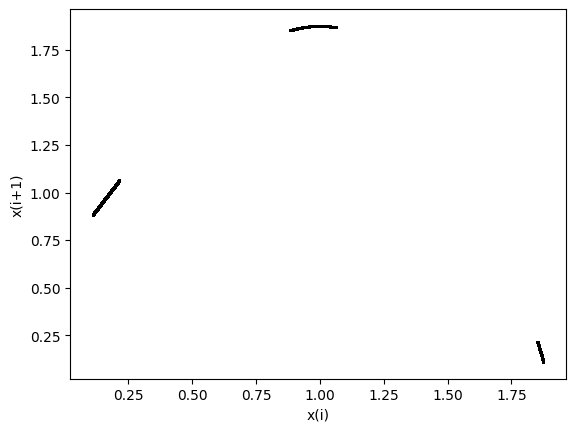
\includegraphics[width=\textwidth]{LateX images/graphs q05/g11}
		\caption{Για k=0.5927}
		\label{f:36}
	\end{subfigure}
		
\end{figure}

 \clearpage

\subsection{Για q=-0.7}

Στο σχήμα \ref{f:g12} παρατίθεται το διάγραμμα διακλάδωσης του συστήματος \ref{f:x1}, ως προς την παράμετρο k, για a=1, b=2 και q =- 0.7. Για αυτές τις τιμές των παραμέτρων το σύστημα ξεκινάει από περίοδο-1 για k = 0.3 αλλά από k[0.3469,0.3486] σπάει η περίοδος. Απο k=3.469 ξαναξεκινάει από περίοδο-1.Για  k = 0.52 εμφανίζει τον πρώτο διπλασιασμό της περιόδου. Τον δεύτερο διπλασιασμό τον εμφανίζει για k=0.57(περίοδος-4) ,τον τρίτο για k=0.592 (περίοδος-8) και τον τέταρτο για k=0.593(περόδος-15).Στην συνέχεια για k>0.593 το σύστημα εισέρχεται στο χάος , μέχρι να εξέλθει  για k=0.627(περίοδος-3) και να ξανά εισέλθει σε χάος μετά από δύο διπλασιασμούς k=0.63 (περίοδος-6)  k=0.631 (περίοδος-11),για k>0.631.
Επομένως και σε αυτή την περίπτωση το σύστημα εισέρχεται στο χάος με διπλασιασμό της περιόδου. 
Επιπλέον, στο σχήμα \ref{f:g11} παρατίθεται το διάγραμμα των εκθετών Lyapunov για τιμές του k στο ίδιο διάστημα τιμών [0, 0.72].  Στο διάστημα τιμών   0<k<0.594 , στο 0.627<k<0.632, παρατηρούμε ότι ο εκθέτης Lyapunov είναι συνεχώς αρνητικός, γεγονός που επιβεβαιώνει την περιοδική συμπεριφορά του συστήματος. Ενώ στα υπόλοιπα διαστήματα ο θετικός εκθέτης Lyapunov υποστηρίζει την χαοτική του συμπεριφορά, όπως έγινε φανερό και από το διάγραμμα διακλάδωσης.
Τέλος, στον Πίνακα \ref{tab:abc3} παρατίθενται ενδεικτικές τιμές της παραμέτρου k και η συμπεριφορά που παρουσιάζει το σύστημα για αυτές, σύμφωνα με το διάγραμμα διακλάδωσης, καθώς και τα αντίστοιχα σχήματα των διαγραμμάτων της τιμής \(x_i\) σε συνάρτηση με την τιμή \(x_{i+1}\). Από τα παραγόμενα σχήματα προκύπτει αριθμός σημείων αντίστοιχος με την περίοδο του συστήματος.

\begin{table}[h!]
	\centering
	\begin{tabular}{l | l | l}
		Παράμετρος k & Συμπεριφορά & Σχήμα\\
		\hline
		0.25 &  Περίοδος-1 & \ref{f:k37}\\
		0.3469&  Περίοδος-1 & \ref{f:k38}\\
		0.52& Περίοδος-2 & \ref{f:k39}\\
		0.57& Περίοδος-4 & \ref{f:k40}\\
		0.592 &  Περίοδος-8 & \ref{f:k41}\\
		0.593& Περίοδος-15 & \ref{f:k42}\\
		0.594 & Χάος & \ref{f:k43}\\
		0.627 & Περίοδος-3 & \ref{f:k44}\\
		0.630 & Περίοδος-6 & \ref{f:k45}\\
		0.631 & Περίοδος-11 & \ref{f:k46}\\
		0.632 & Χάος & \ref{f:k47}\\
	\end{tabular}
	\caption{ Συμπεριφορά του υπό μελέτη συστήματος για διάφορες τιμές του k,για a=1, b=2 και q=-0.7}
	\label{tab:abc3}
\end{table}

\begin{figure}[h!]
	\centering
	\includegraphics[width=0.6\linewidth]{LateX images/graphs q07/g1}
	\caption{ Διάγραμμα διακλάδωσης, για a=1, b=2 και q=-0.7}
	\label{f:g12}
\end{figure}
\begin{figure}[h!]
	\centering
	\includegraphics[width=0.6\linewidth]{"LateX images/graphs q07/g2 "}
	\caption{Διάγραμμα του εκθέτη Lyapunov σε συνάρτηση με την παράμετρο k, για a=1, b=2 και q=-0.7.}
	\label{f:g13}
\end{figure}

\begin{figure}[h!]
	\centering
	\caption{Διαγράμματα της τιμής \(x_i\) με την τιμή \(x_{i+1}\) :}
	\begin{subfigure}[b]{0.25\textwidth}
		\centering
		\includegraphics[width=\textwidth]{LateX images/graphs q07/g3}
		\caption{Για k=0.25}
		\label{f:k37}
	\end{subfigure}
	\hfill
	\begin{subfigure}[b]{0.25\textwidth}
		\centering
		\includegraphics[width=\textwidth]{LateX images/graphs q07/g4}
		\caption{Για k=0.3469}
		\label{f:k38}
	\end{subfigure}
	\hfill
	\begin{subfigure}[b]{0.25\textwidth}
		\centering
		\includegraphics[width=\textwidth]{LateX images/graphs q07/g5}
		\caption{Για k=0.52}
		\label{f:k39}
	\end{subfigure}
	\begin{subfigure}[b]{0.25\textwidth}
		\centering
		\includegraphics[width=\textwidth]{LateX images/graphs q07/g6}
		\caption{Για k=0.57}
		\label{f:k40}
	\end{subfigure}
	\hfill
	\begin{subfigure}[b]{0.25\textwidth}
		\centering
		\includegraphics[width=\textwidth]{LateX images/graphs q07/g7}
		\caption{Για k=0.592}
		\label{f:k41}
	\end{subfigure}
	\hfill
	\begin{subfigure}[b]{0.25\textwidth}
		\centering
		\includegraphics[width=\textwidth]{LateX images/graphs q07/g8}
		\caption{Για k=0.593}
		\label{f:k42}
	\end{subfigure}
	\hfill
	\begin{subfigure}[b]{0.25\textwidth}
		\centering
		\includegraphics[width=\textwidth]{LateX images/graphs q07/g9}
		\caption{Για k=0.594}
		\label{f:k43}
	\end{subfigure}
	\hfill
	\begin{subfigure}[b]{0.25\textwidth}
		\centering
		\includegraphics[width=\textwidth]{LateX images/graphs q07/g10}
		\caption{Για k=0.627}
		\label{f:k44}
	\end{subfigure}
	\hfill
	\begin{subfigure}[b]{0.25\textwidth}
		\centering
		\includegraphics[width=\textwidth]{LateX images/graphs q07/g11}
		\caption{Για k=0.63}
		\label{f:k45}
	\end{subfigure}
	\hfill
	\begin{subfigure}[b]{0.25\textwidth}
		\centering
		\includegraphics[width=\textwidth]{LateX images/graphs q07/g12}
		\caption{Για k=0.631}
		\label{f:k46}
	\end{subfigure}
	\hfill
	\begin{subfigure}[b]{0.25\textwidth}
	\centering
	\includegraphics[width=\textwidth]{LateX images/graphs q07/g13}
	\caption{Για k=0.632}
	\label{f:k47}
	\end{subfigure}
	
\end{figure}

\clearpage

\subsection{Για q=-0.9}

\begin{table}[h!]
	\centering
	\begin{tabular}{l | l | l}
		Παράμετρος k & Συμπεριφορά & Σχήμα\\
		\hline
		0.43 &  Περίοδος-1 & \ref{f:k48}\\
		0.436 &  Περίοδος-1 & \ref{f:k49}\\
		0.57& Περίοδος-2 & \ref{f:k50}\\
		0.62& Περίοδος-4 & \ref{f:k51}\\
		0.63 &  Περίοδος-8 & \ref{f:k52}\\
		0.633& Περίοδος-16 & \ref{f:k53}\\
		0.635& Χάος & \ref{f:k54}\\
		0.665 & Περίοδος-3 & \ref{f:k55}\\
		0.668 & Περίοδος-6 & \ref{f:k56}\\
		0.671 & Χάος & \ref{f:k57}\\
		0.72 & Περίοδος-1& \ref{f:k58}\\
	\end{tabular}
	\caption{ Συμπεριφορά του υπό μελέτη συστήματος για διάφορες τιμές του k,για a=1, b=2 και q=-0.9}
	\label{tab:abc4}
\end{table}

\begin{figure}[h!]
	\centering
	\includegraphics[width=0.6\linewidth]{LateX images/graphs q09/g1}
	\caption{ Διάγραμμα διακλάδωσης, για a=1, b=2 και q=-0.9}
	\label{f:g14}
\end{figure}

\begin{figure}[h!]
	\centering
	\includegraphics[width=0.6\linewidth]{LateX images/graphs q09/g2}
	\caption{Διάγραμμα του εκθέτη Lyapunov σε συνάρτηση με την παράμετρο k, για a=1, b=2 και q=-0.9}
	\label{f:g15}
\end{figure}

\begin{figure}[h!]
	\centering
	\caption{Διαγράμματα της τιμής \(x_i\) με την τιμή \(x_{i+1}\) :}
	\begin{subfigure}[b]{0.25\textwidth}
		\centering
		\includegraphics[width=\textwidth]{LateX images/graphs q09/g3}
		\caption{Για k=0.43}
		\label{f:k48}
	\end{subfigure}
	\hfill
	\begin{subfigure}[b]{0.25\textwidth}
		\centering
		\includegraphics[width=\textwidth]{LateX images/graphs q09/g4}
		\caption{Για k=0.436}
		\label{f:k49}
	\end{subfigure}
	\hfill
	\begin{subfigure}[b]{0.25\textwidth}
		\centering
		\includegraphics[width=\textwidth]{LateX images/graphs q09/g5}
		\caption{Για k=0.57}
		\label{f:k50}
	\end{subfigure}
	\begin{subfigure}[b]{0.25\textwidth}
		\centering
		\includegraphics[width=\textwidth]{LateX images/graphs q09/g6}
		\caption{Για k=0.62}
		\label{f:k51}
	\end{subfigure}
	\hfill
	\begin{subfigure}[b]{0.25\textwidth}
		\centering
		\includegraphics[width=\textwidth]{LateX images/graphs q09/g13}
		\caption{Για k=0.63}
		\label{f:k52}
	\end{subfigure}
	\hfill
	\begin{subfigure}[b]{0.25\textwidth}
		\centering
		\includegraphics[width=\textwidth]{LateX images/graphs q09/g7}
		\caption{Για k=0.633}
		\label{f:k53}
	\end{subfigure}
	\hfill
	\begin{subfigure}[b]{0.25\textwidth}
		\centering
		\includegraphics[width=\textwidth]{LateX images/graphs q09/g8}
		\caption{Για k=0.635}
		\label{f:k54}
	\end{subfigure}
	\hfill
	\begin{subfigure}[b]{0.25\textwidth}
		\centering
		\includegraphics[width=\textwidth]{LateX images/graphs q09/g9}
		\caption{Για k=0.665}
		\label{f:k55}
	\end{subfigure}
	\hfill
	\begin{subfigure}[b]{0.25\textwidth}
		\centering
		\includegraphics[width=\textwidth]{LateX images/graphs q09/g10}
		\caption{Για k=0.668}
		\label{f:k56}
	\end{subfigure}
	\hfill
	\begin{subfigure}[b]{0.25\textwidth}
		\centering
		\includegraphics[width=\textwidth]{LateX images/graphs q09/g11}
		\caption{Για k=0.671}
		\label{f:k57}
	\end{subfigure}
	\hfill
	\begin{subfigure}[b]{0.25\textwidth}
		\centering
		\includegraphics[width=\textwidth]{LateX images/graphs q09/g12}
		\caption{Για k=0.72}
		\label{f:k58}
	\end{subfigure}
	\hfill
	
\end{figure}

\clearpage

\subsection{Για q=-1.2}

\begin{table}[h!]
	\centering
	\begin{tabular}{l | l | l}
		Παράμετρος k & Συμπεριφορά & Σχήμα\\
		\hline
		0.55 &  Περίοδος-1 & \ref{f:k59}\\
		0.566 &  Περίοδος-1 & \ref{f:k60}\\
		0.63& Περίοδος-2 & \ref{f:k61}\\
		0.68& Περίοδος-4 & \ref{f:k62}\\
		0.69 &  Περίοδος-8 & \ref{f:k63}\\
		0.696& Χάος & \ref{f:k64}\\
		0.726& Περίοδος-3 & \ref{f:k65}\\
		0.729& Περίοδος-6 & \ref{f:k66}\\
		0.731& Χάος & \ref{f:k67}\\
		0.762 &  Περίοδος-1 & \ref{f:k68}\\
	\end{tabular}
	\caption{ Συμπεριφορά του υπό μελέτη συστήματος για διάφορες τιμές του k,για a=1, b=2 και q=-0.9}
	\label{tab:abc5}
\end{table}

\begin{figure}[h!]
	\centering
	\includegraphics[width=0.6\linewidth]{LateX images/graphs q12/g1}
	\caption{ Διάγραμμα διακλάδωσης, για a=1, b=2 και q=-1.2}
	\label{f:g16}
\end{figure}

\begin{figure}[h!]
	\centering
	\includegraphics[width=0.6\linewidth]{LateX images/graphs q12/g2}
	\caption{Διάγραμμα του εκθέτη Lyapunov σε συνάρτηση με την παράμετρο k, για a=1, b=2 και q=-1.2}
	\label{f:g17}
\end{figure}

\begin{figure}[h!]
	\centering
	\caption{Διαγράμματα της τιμής \(x_i\) με την τιμή \(x_{i+1}\) :}
	\begin{subfigure}[b]{0.25\textwidth}
		\centering
		\includegraphics[width=\textwidth]{LateX images/graphs q12/g3}
		\caption{Για k=0.55}
		\label{f:k59}
	\end{subfigure}
	\hfill
	\begin{subfigure}[b]{0.25\textwidth}
		\centering
		\includegraphics[width=\textwidth]{LateX images/graphs q12/g4}
		\caption{Για k=0.566}
		\label{f:k60}
	\end{subfigure}
	\hfill
	\begin{subfigure}[b]{0.25\textwidth}
		\centering
		\includegraphics[width=\textwidth]{LateX images/graphs q12/g5}
		\caption{Για k=0.63}
		\label{f:k61}
	\end{subfigure}
	\begin{subfigure}[b]{0.25\textwidth}
		\centering
		\includegraphics[width=\textwidth]{LateX images/graphs q12/g6}
		\caption{Για k=0.68}
		\label{f:k62}
	\end{subfigure}
	\hfill
	\begin{subfigure}[b]{0.25\textwidth}
		\centering
		\includegraphics[width=\textwidth]{LateX images/graphs q12/g7}
		\caption{Για k=0.69}
		\label{f:k63}
	\end{subfigure}
	\hfill
	\begin{subfigure}[b]{0.25\textwidth}
		\centering
		\includegraphics[width=\textwidth]{LateX images/graphs q12/g8}
		\caption{Για k=0.696}
		\label{f:k64}
	\end{subfigure}
	\hfill
	\begin{subfigure}[b]{0.25\textwidth}
		\centering
		\includegraphics[width=\textwidth]{LateX images/graphs q12/g9}
		\caption{Για k=0.726}
		\label{f:k65}
	\end{subfigure}
	\hfill
	\begin{subfigure}[b]{0.25\textwidth}
		\centering
		\includegraphics[width=\textwidth]{LateX images/graphs q12/g10}
		\caption{Για k=0.729}
		\label{f:k66}
	\end{subfigure}
	\hfill
	\begin{subfigure}[b]{0.25\textwidth}
		\centering
		\includegraphics[width=\textwidth]{LateX images/graphs q12/g11}
		\caption{Για k=0.731}
		\label{f:k67}
	\end{subfigure}
	\hfill
	\begin{subfigure}[b]{0.25\textwidth}
		\centering
		\includegraphics[width=\textwidth]{LateX images/graphs q12/g12}
		\caption{Για k=0.762}
		\label{f:k68}
	\end{subfigure}
	\hfill
	
\end{figure}

\clearpage

\subsection{Για q=-1.4}

\begin{table}[h!]
	\centering
	\begin{tabular}{l | l | l}
		Παράμετρος k & Συμπεριφορά & Σχήμα\\
		\hline
		0.5 &  Περίοδος-1 & \ref{f:k59}\\
		0.54 &  Περίοδος-2 & \ref{f:k60}\\
		0.65& Περίοδος-1 & \ref{f:k61}\\
		0.68& Περίοδος-2 & \ref{f:k62}\\
		0.725 &  Περίοδος-4 & \ref{f:k63}\\
		0.735& Περίοδος-8 & \ref{f:k64}\\
		0.737& Περίοδος-15 & \ref{f:k65}\\
		0.738& Χάος & \ref{f:k66}\\
		0.767 &  Περίοδος-3& \ref{f:k68}\\
		0.769 &  Περίοδος-6& \ref{f:k68}\\
		0.77 &  Χάος& \ref{f:k68}\\
		0.8 &  Περίοδος-2& \ref{f:k68}\\
		
	\end{tabular}
	\caption{ Συμπεριφορά του υπό μελέτη συστήματος για διάφορες τιμές του k,για a=1, b=2 και q=-0.9}
	\label{tab:abc6}
\end{table}

[0,0.91]


\chapter{Κεφάλαιο 3}
Στο κεφάλαιο αυτό παρουσιάζεται αναλυτικά η μελέτη της δυναμικής συμπεριφοράς ενός διακριτού συστήματος που αποτελεί παραλλαγή του γνωστού \emph{sine-sinh-sine} Χάρτη. Για επιλεγμένες τιμές της παραμέτρου του μπορεί να παρουσιάσει χαοτική συμπεριφορά όπως και φαινόμενα που σχετίζονται με τη μη-γραμμική δυναμική. Για τη μελέτη χρησιμοποιήθηκαν τα διαγράμματα διακλάδωσης, οι εκθέτες Lyapunov και οι απεικονίσεις της τιμής \(x_i\) σε συνάρτηση με  την τιμή \(x_{i+1}\).

Ο \emph{sine-sinh-sine} Χάρτης που αποτέλεσε τη βάση του προτεινόμενου σε αυτή την ενότητα, χάρτη, περιγράφεται από την παρακάτω εξίσωση \cite{b10}:

\begin{equation}
	x_{i+1}=k*\sin(\pi*\sinh(\pi*\sin(\pi* x_i)))
	\label{f:x2}
\end{equation}


Στην εξίσωση (\ref{f:x2})αντικαταστάθηκε η παράμετρος $\pi$
με την παράμετρο k, ένα σταθερό όρο q και έναν ακέραιο αριθμό. Έτσι προέκυψε η προτεινόμενη παραλλαγή του Λογιστικού Χάρτη,

\begin{equation}
	x_{i+1}=k*\sin(k*\sinh(q*\sin(2 * x_i)))
	\label{f:x3}
\end{equation}
όπου k, q παράμετροι.\\

Για την εύρεση της δυναμικής συμπεριφοράς του συστήματος (3.2) εξετάστηκε μια περιοχή τιμών των συγκεκριμένων παραμέτρων. Πιο συγκεκριμένα, στη μελέτη που πραγματοποιήθηκε η αρχική συνθήκη του συστήματος ($x_0 =0.1$) παρέμεινε  σταθερή, ενώ η τιμή της παραμέτρου q μεταβαλλόταν στο διάστημα $[-0.3,-0.5]$ με βήμα $0.2$. Έτσι, για κάθε περίπτωση παράχθηκαν το διάγραμμα διακλάδωσης, το διάγραμμα των εκθετών Lyapunov και το διάγραμμα της τιμής \(x_i\) σε συνάρτηση με  την τιμή \(x_{i+1}\), τα οποία παρουσιάζονται και αναλύονται στη συνέχεια.\\


\vspace{\fill}

\section{Για \emph{q} = -0.3}


Στo Σχ. \ref{f:g44} παρατίθεται τα διάγραμμα διακλάδωσης του συστήματος (\ref{f:x3}), ως προς την παράμετρο k, για $q =- 0.3$. 
Στον πίνακα \ref{tab:abc10} φαίνεται η πορεία του συστήματος και για ποιες τιμές της παραμέτρου k το σύστημα εμφανίζει περιοδική ή χαοτική συμπεριφορά, σύμφωνα με το διάγραμμα διακλάδωσης του Σχ. \ref{f:g44}. Επίσης παρατηρείται συνοριακή κρίση ελκυστών για διάφορες τιμές του k (2.27, 2.31, 2.43, 2.671, 2.76, 2.935, 3.293, 3.48, 3.629, 3.79), το οποίο φαίνεται ξεκάθαρα στο διάγραμμα διακλάδωσης του Σχ. \ref{f:g44}, στην μεταπήδηση του συστήματος από χαοτική συμπεριφορά σε \emph{περίοδο - 1} και \emph{περίοδο - 2}. Οι αντίστοιχες τιμές του k για αυτά τα σημεία του διαγράμματος υπάρχουν στο Πίνακα \ref{tab:abc10}, όπως και τα αντίστοιχα διαγράμματα της τιμής \(x_i\) σε συνάρτηση με την τιμή \(x_{i+1}\) του Σχ. \ref{f:k246}. Από τα παραγόμενα σχήματα προκύπτει αριθμός σημείων αντίστοιχος με την περίοδο του συστήματος.

Τέλος, στο Σχ. \ref{f:g45} παρατίθεται το διάγραμμα των εκθετών Lyapunov για τιμές του k στο ίδιο διάστημα τιμών $[0, 4.2]$. Οι τιμές του Πίνακα \ref{tab:abc10} που έχουν περιοδική συμπεριφορά αντιστοιχούν σε τιμές του διαγράμματος του Σχ. \ref{f:g44}, όπου o εκθέτης Lyapunov είναι συνεχώς αρνητικός, γεγονός που επιβεβαιώνει την συμπεριφορά του. Ενώ για τις υπόλοιπες τιμές ο θετικός εκθέτης Lyapunov υποστηρίζει τη χαοτική του συμπεριφορά, όπως γίνεται φανερό και από το διάγραμμα διακλάδωσης.\\\\

\begin{figure}[ht]
	\centering
	\includegraphics[width=1\linewidth]{LateX images/sine q=-0.3/g1}
	\caption{Διάγραμμα διακλάδωσης, για $q=-0.3$.}
	\label{f:g44}
\end{figure}



\begin{table}[ht]
	\centering
	\caption{ Συμπεριφορά του υπό μελέτη συστήματος για διάφορες τιμές του k, για $q=-0.3$ }
	\label{tab:abc10}
	\begin{tabular}{l | l}
		Παράμετρος k & Συμπεριφορά \\
		\hline
		0.25 &  Περίοδος -  1 \\
		1.287 &  Περίοδος -  2 \\
		2.17& Περίοδος -  4 \\
		2.2& Περίοδος -  8 \\
		2.21 & Xάος \\
		2.27& Περίοδος - 10 \\
		2.272& Χάος \\
		2.31& Περίοδος - 6 \\
		2.32 &  Χάος \\
		2.43 &  Περίοδος -  3 \\
		2.435 &  Χάος \\
		2.671 &  Περίοδος -  3\\
		2.672 & Περίοδος - 6\\
		2.675 & Χάος\\
		2.76 &Περίοδος - 6 \\
		2.77& Χάος\\
		2.935 & Περίοδος -  1\\
		3.14& Περίοδος - 2\\
		3.22 & Περίοδος -  4\\
		3.79 &Περίοδος - 4\\
		3.8 & Χάος\\
		4.09& Περίοδος - 2
		
	\end{tabular}
	
\end{table}


\begin{figure}[ht]
	\centering
	\includegraphics[width=1\linewidth]{LateX images/sine q=-0.3/g2}
	\caption{Διάγραμμα των εκθετών Lyapunov σε συνάρτηση με την παράμετρο k, για $q=-0.3$.}
	\label{f:g45}
\end{figure}



\begin{figure}[ht]
	\centering
	\begin{subfigure}[b]{0.4\textwidth}
		\centering
		\includegraphics[width=\textwidth]{LateX images/sine q=-0.3/g3}
		\caption{Για $k=2.27$}
		\label{f:k116}
	\end{subfigure}
	\hfill
	\begin{subfigure}[b]{0.4\textwidth}
		\centering
		\includegraphics[width=\textwidth]{LateX images/sine q=-0.3/g4}
		\caption{Για $k=2.31$}
		\label{f:k117}
	\end{subfigure}
	\hfill
	\begin{subfigure}[b]{0.4\textwidth}
		\centering
		\includegraphics[width=\textwidth]{LateX images/sine q=-0.3/g5}
		\caption{Για $k=2.43$}
		\label{f:k118}
	\end{subfigure}
	\hfill
	\begin{subfigure}[b]{0.4\textwidth}
		\centering
		\includegraphics[width=\textwidth]{LateX images/sine q=-0.3/g6}
		\caption{Για $k=2.671$}
		\label{f:k119}
	\end{subfigure}
	\hfill
	\begin{subfigure}[b]{0.4\textwidth}
		\centering
		\includegraphics[width=\textwidth]{LateX images/sine q=-0.3/g7}
		\caption{Για $k=2.76$}
		\label{f:k120}
	\end{subfigure}
	\hfill
	\begin{subfigure}[b]{0.4\textwidth}
		\centering
		\includegraphics[width=\textwidth]{LateX images/sine q=-0.3/g20}
		\caption{Για $k=3.8$}
		\label{f:k126}
	\end{subfigure}
	\hfill		
	\caption{Διαγράμματα της τιμής \(x_i\) σε συνάρτηση με την τιμή \(x_{i+1}\).}
	\label{f:k246}
\end{figure}

\clearpage 
\section{Για \emph{q} = -0.5}

Στο Σχ. \ref{f:48} παρατίθενται τα διαγράμματα διακλάδωσης του συστήματος \ref{f:x3}, ως προς την παράμετρο k, για $q =-0.5$ και για διαφορετικές αρχικές συνθήκες, δηλαδή για διαφορετικό \(x_0\). Συγκρίνοντας το διάγραμμα του Σχ. \ref{f:g46} (\(x_0=0.1\)) με τα υπόλοιπα διαγράμματα διακλάδωσης των Σχ. \ref{f:g47} (\(x_0=0.5\)), \ref{f:g48} (\(x_0=1\)), παρατηρείται ότι για $q=-0.5$ εμφανίζεται το φαινόμενο της συνύπαρξης ελκυστών. Η συμπεριφορά του συστήματος για τις διάφορες περιπτώσεις επιβεβαιώνεται και από τα αντίστοιχα διαγράμματα Lyapunov των Σχ. (\ref{f:g49}, \ref{f:g50}, \ref{f:g51}), όπως και απο το διάγραμμα διακλάδωσης του Σχ. \ref{f:g54}, όπου η κάθε αρχική συνθήκη εμφανίζεται με διαφορετικό χρώμα.

Στον Πίνακα \ref{tab:abc11} φαίνεται η πορεία του συστήματος και για ποιες τιμές της παραμέτρου k το σύστημα εμφανίζει περιοδική ή χαοτική συμπεριφορά, σύμφωνα με το διάγραμμα διακλάδωσης του Σχ. \ref{f:g46}. Οι τιμές αυτές αντιστοιχούν στα σχήματα των διαγραμμάτων της τιμής \(x_i\) σε συνάρτηση με την τιμή \(x_{i+1}\). Από τα παραγόμενα Σχ. \ref{f:g58} προκύπτει αριθμός σημείων αντίστοιχος με την περίοδο του συστήματος.

Επίσης παρατηρείται η συνοριακή κρίση ελκυστών για διάφορες τιμές του k (1.773, 1.8, 1.831, 1.93, 2.03, 2.141, 2.2, 2.38,
2.88, 2.99, 3.04, 3.2, 3.35, 3.4, 3.44, 3.62, 3.93), όπως και το φαινόμενο της υστέρησης το οποίο διακρίνεται στα κενά που δημιουργούνται στις σκιαγραφημένες περιοχές 1 και 2. Οι αντίστοιχες τιμές του k για αυτά τα σημεία του διαγράμματος υπάρχουν στο Πίνακα \ref{tab:abc11}.

Επιπλέον παρατηρούμε στα διαγράμματα των Σχ. \ref{f:g237}, \ref{f:g238}, \ref{f:g239} το φαινόμενο της αντιμονοτονικότητας. Συγκεκριμένα στα διαγράμματα του Σχ. \ref{f:g237} εμφανίζεται μία χαοτική φυσαλίδα (το σύστημα εισέρχεται στο χάος με διπλασιασμό της περιόδου και στη συνέχεια εξέρχεται από αυτό με ανάστροφη ακολουθία διπλασιασμού της περιόδου), για $k=3.85$, της οποίας η εξέλιξη φαίνεται στα υπόλοιπα δύο διαγράμματα των. Σχ. \ref{f:g238}, \ref{f:g239}, όπου για διαφορετικές αρχικές συνθήκες $x_0$ διακρίνεται καλύτερα.
Μεταξύ αυτών των χαοτικών φυσαλίδων παρατηρούμε και τις δύο περιπτώσεις του φαινομένου, δηλαδή τον ορθό και τον ανάστροφο διπλασιασμό της περιόδου. Στα Σχ. \ref{f:g238}, \ref{f:g239} παρατηρείται ότι για $k=3.95$ ξεκινάει η ανάστροφη φυσαλίδα με \emph{περίοδο-1}.

Τέλος, στο σχήμα \ref{f:g49} παρατίθεται το διάγραμμα των εκθετών Lyapunov για τιμές του k στο ίδιο διάστημα τιμών $[0, 4.2]$. Οι τιμές του Πίνακα \ref{tab:abc11} που έχουν περιοδική συμπεριφορά αντιστοιχούν σε τιμές του διαγράμματος του Σχ. \ref{f:g49}, όπου ο εκθέτης Lyapunov είναι συνεχώς αρνητικός, γεγονός που επιβεβαιώνει την συμπεριφορά τους. Ενώ για τις υπόλοιπες τιμές ο θετικός εκθέτης Lyapunov υποστηρίζει την χαοτική τους συμπεριφορά, όπως γίνεται φανερό και από το διάγραμμα διακλάδωσης.





\begin{table}[ht]
	\centering
	\caption{ Συμπεριφορά του υπό μελέτη συστήματος για διάφορες τιμές του k, για $q=-0.5$ }
	\label{tab:abc11}
	\begin{tabular}{l | l}
		Παράμετρος k & Συμπεριφορά \\
		\hline
		0.25 &  Περίοδος -  1 \\
		1 &  Περίοδος -  2 \\
		1.7& Περίοδος -  4 \\
		1.748& Περίοδος -  8 \\
		1.75 & Xάος \\
		1.773& Περίοδος - 6 \\
		1.774& Περίοδος - 12\\
		1.775& Χάος \\
		1.8& Περίοδος - 10 \\
		1.806 &  Χάος \\
		2.03 &  Περίοδος -  4\\
		2.06 &Χάος \\
		2.88& Περίοδος -  3\\
		2.89 & Χάος\\
		2.99 &  Περίοδος -  6\\
		3 &  Περίοδος - 12\\
		3.01 &  Χάος\\
		3.04 & Περίοδος - 4\\
		3.08 & Χάος\\
		3.2 & Περίοδος -2\\
		3.206 & Περίοδος -  4\\
		3.23 & Περίοδος -  2\\
		3.24 & Χάος\\
		3.35 & Περίοδος -  4\\
		3.36 & Χάος\\
		3.4 & Περίοδος -  4\\
		3.41 & Χάος\\
		3.44 & Περίοδος -  4\\
		3.45 & Χάος\\
		3.62 & Περίοδος -  2\\
		3.8 & Περίοδος -  4\\
		3.84 & Χάος\\
		3.94 & Περίοδος -  8\\
		3.95 & Περίοδος -  4\\
		3.96 & Περίοδος -  8\\
		3.97 & Περίοδος -  16\\
		3.98 & Χάος\\
		4 & Περίοδος -  6\\
		4.05&Περίοδος - 4\\
		4.07 & Χάος\\
		
	\end{tabular}
	
\end{table}


\begin{figure}[ht]
	\centering
	\begin{subfigure}[b]{0.8\textwidth}
		\centering
		\includegraphics[width=\textwidth]{LateX images/sine q=-0.5/g4}
		\caption{\(x_0=0.1\)}
		\label{f:g46}
	\end{subfigure}
	\hfill
	\begin{subfigure}[b]{0.8\textwidth}
		\centering
		\includegraphics[width=\textwidth]{LateX images/sine q=-0.5/g5}
		\caption{\(x_0=0.5\)}
		\label{f:g47}
	\end{subfigure}
	\hfill
	\begin{subfigure}[b]{0.8\textwidth}
		\centering
		\includegraphics[width=\textwidth]{LateX images/sine q=-0.5/g6}
		\caption{\(x_0=1\)}
		\label{f:g48}
	\end{subfigure}
	\caption{ Διαγράμματα διακλάδωσης, για $q=-0.5$}
	\label{f:48}
\end{figure}

\begin{figure}[ht]
	\centering
	
	\begin{subfigure}[b]{0.8\textwidth}
		\centering
		\includegraphics[width=\textwidth]{LateX images/sine q=-0.5/g8}
		\caption{Για \(x_0=0.1\)}
		\label{f:g49}
	\end{subfigure}
	\hfill
	\begin{subfigure}[b]{0.8\textwidth}
		\centering
		\includegraphics[width=\textwidth]{LateX images/sine q=-0.5/g9}
		\caption{Για \(x_0=0.5\)}
		\label{f:g50}
	\end{subfigure}
	\hfill
	\begin{subfigure}[b]{0.8\textwidth}
		\centering
		\includegraphics[width=\textwidth]{LateX images/sine q=-0.5/g10}
		\caption{Για \(x_0=1\)}
		\label{f:g51}
	\end{subfigure}
	\hfill
	\caption{ Διαγράμματα των εκθετών Lyapunov σε συνάρτηση με την παράμετρο k, για $q=-0.5$.}
	\label{f:g236}
\end{figure}



\begin{figure}[ht]
	\centering
	
	\begin{subfigure}[b]{0.8\textwidth}
		\centering
		\includegraphics[width=\textwidth]{LateX images/sine q=-0.5/g3}
		\caption{Περιοχή 1 (βλ. Σχ. \ref{f:g46})}
		\label{f:g52}
	\end{subfigure}
	\hfill
	\begin{subfigure}[b]{0.8\textwidth}
		\centering
		\includegraphics[width=\textwidth]{LateX images/sine q=-0.5/g3.2}
		\caption{Περιοχή 2 (βλ. Σχ. \ref{f:g46})}
		\label{f:g533}
	\end{subfigure}
	
	\caption{Διαγράμματα διακλάδωσης για διάφορες τιμές του $x_0=0.1$. }
	\label{f:g237}
\end{figure}
\begin{figure}[ht]
	\centering	
	\begin{subfigure}[b]{0.8\textwidth}
		\centering
		\includegraphics[width=\textwidth]{LateX images/sine q=-0.5/g7}
		\caption{Περιοχή 1 (βλ. Σχ. \ref{f:g47})}
		\label{f:g522}
	\end{subfigure}
	\hfill
	\begin{subfigure}[b]{0.8\textwidth}
		\centering
		\includegraphics[width=\textwidth]{LateX images/sine q=-0.5/g7.2}
		\caption{Περιοχή 2 βλ. Σχ. \ref{f:g47})}
		\label{f:g523}
	\end{subfigure}
	\caption{Διαγράμματα διακλάδωσης για διάφορες τιμές του $x_0=0.5$. }
	\label{f:g238}
\end{figure}
\begin{figure}[ht]
	\centering
	
	\begin{subfigure}[b]{0.8\textwidth}
		\centering
		\includegraphics[width=\textwidth]{LateX images/sine q=-0.5/g12}
		\caption{Περιοχή 1 (βλ. Σχ. \ref{f:g48})}
		\label{f:g524}
	\end{subfigure}
	\hfill
	\begin{subfigure}[b]{0.8\textwidth}
		\centering
		\includegraphics[width=\textwidth]{LateX images/sine q=-0.5/g12.2}
		\caption{Περιοχή 2 (βλ. Σχ. \ref{f:g48})}
		\label{f:g525}
	\end{subfigure}
	\caption{Διαγράμματα διακλάδωσης για διάφορες τιμές του $x_0=1$. }
	\label{f:g239}
\end{figure}

\begin{figure}[ht]
	\centering
	
	\begin{subfigure}[b]{0.8\textwidth}
		\centering
		\includegraphics[width=\textwidth]{LateX images/sine q=-0.5/g2}
		\caption{$x_0=0.1$}
		\label{f:g54}
	\end{subfigure}
	\hfill
	\begin{subfigure}[b]{0.8\textwidth}
		\centering
		\includegraphics[width=\textwidth]{LateX images/sine q=-0.5/g14}
		\caption{$x_0=0.5$}
		\label{f:g55}
	\end{subfigure}
	\begin{subfigure}[b]{0.8\textwidth}
		\centering
		\includegraphics[width=\textwidth]{LateX images/sine q=-0.5/g15}
		\caption{$x_0=1$}
		\label{f:g56}
	\end{subfigure}
	
	\caption{Διαγράμματα διακλάδωσης για διάφορες τιμές του $x_0$. }
\end{figure}

\begin{figure}[ht]
	\centering
	\includegraphics[width=1\linewidth]{LateX images/sine q=-0.5/g11}
	\caption{Διάγραμμα διακλάδωσης, για όλες τις διαφορετικές αρχικές συνθήκες $x_0$.}
	\label{f:g57}
\end{figure}

\begin{figure}[ht]
	\centering
	\begin{subfigure}[b]{0.4\textwidth}
		\centering
		\includegraphics[width=\textwidth]{LateX images/sine q=-0.5/g16}
		\caption{Για $k=1.775$}
		\label{f:k127}
	\end{subfigure}
	\hfill
	\begin{subfigure}[b]{0.4\textwidth}
		\centering
		\includegraphics[width=\textwidth]{LateX images/sine q=-0.5/g17}
		\caption{Για $k=2.03$}
		\label{f:k128}
	\end{subfigure}
	\hfill
	\begin{subfigure}[b]{0.4\textwidth}
		\centering
		\includegraphics[width=\textwidth]{LateX images/sine q=-0.5/g19}
		\caption{Για $k=2.84$}
		\label{f:k129}
	\end{subfigure}
	\hfill
	\begin{subfigure}[b]{0.4\textwidth}
		\centering
		\includegraphics[width=\textwidth]{LateX images/sine q=-0.5/g18}
		\caption{Για $k=3$}
		\label{f:k130}
	\end{subfigure}
	\hfill
	\begin{subfigure}[b]{0.4\textwidth}
		\centering
		\includegraphics[width=\textwidth]{LateX images/sine q=-0.5/g20}
		\caption{Για $k=3.01$}
		\label{f:k131}
	\end{subfigure}
	\hfill
	\begin{subfigure}[b]{0.4\textwidth}
		\centering
		\includegraphics[width=\textwidth]{LateX images/sine q=-0.5/g21}
		\caption{Για $k=4$}
		\label{f:k132}
	\end{subfigure}
	\hfill			
	\caption{Διαγράμματα της τιμής \(x_i\) σε συνάρτηση με την τιμή \(x_{i+1}\).}
	\label{f:g58}
\end{figure}

\clearpage

\section{Συμπεράσματα}

Σε αυτό το κεφάλαιο παρουσιάστηκε μία παραλλαγή του \emph{sine-sinh-sine} Χάρτη, της οποίας βασικό χαρακτηριστικό είναι η χαοτική συμπεριφορά που καταγράφηκε σε όλες τις περιπτώσεις που ελέγχθηκαν για την παράμετρο q, όπως και για τα επί μέρους φαινόμενα που οδηγούν σε αυτήν.

Ειδικότερα, το συνηθέστερο φαινόμενο που παρατηρήθηκε σε όλες τις περιπτώσεις είναι αυτό της μετάβασης στο χάος μέσω του διπλασιασμού της περιόδου, ξεκινώντας απο διάστημα \emph{περιόδου-1}.
Για κάποιες παραμέτρους  q εμφανίστηκε η ανάστροφη πορεία του συστήματος κατά την έξοδο του απο την χαοτική περιοχή, παρουσιάζοντας έτσι το φαινόμενο της αντιμονοτονικότητας (χαοτική φυσαλίδα).
Επίσης αρκετές φορές παρατηρήθηκε το φαινόμενο της υστέρησης δηλαδή "έσπαγε" η περιοδική συμπεριφορά, καθώς και το φαινόμενο των κρίσεων είτε εσωτερικών, είτε συνοριακών. Τέλος, παρατηρήθηκε το φαινόμενο της συνύπαρξης ελκυστών. 
\newpage

\appendix

\chapter{Appendix title}


Η Python τα τελευταία χρόνια χρησιμοποιείται όλο και περισσότερο στον κόσμο του προγραμματισμού  και κυρίως στους επιστημονικούς κύκλους. Δίνεται η επιλογή στον ερευνητή να χρησιμοποιήσει απείρες βιβλιοθήκες οι οποίες είναι κατάλληλες ακόμα και για τα πιο εξιδεικευμένα έργα. Είναι αρκετά εύπλαστη, ένα προτέρημα που την κάνει να ξεχωρίζει από παλιότερες γλώσσες προγραμματισμού. Επίσης όλα τα παραπάνω την κάνουν αρκετά προσιτή σε οποιοδήποτε άτομο θέλει να ξεκινήσει να ασχολείται με τον προγραμματισμό, χωρίς να έχει προηγούμενη εμπειρία στο αντικείμενο.

Οι κώδικες που γράφτηκαν για την μελέτη τόσο των διακριτών χαοτικών συστημάτων, όσο και για την εφαρμογή τους στον έλεγχο της κίνησης του ρομποτικού οχήματος, παρατίθενται στη συνέχεια.

\lstinputlisting[language=Python,caption=Bifurcation Diagram]{chapters/python/Bifurcation diagram.py}

\lstinputlisting[language=Python,caption=Lyapunov expotent]{chapters/python/Lyapunov expotent.py}

\lstinputlisting[language=Python,caption=$x_i-x_i+1$ diagram]{chapters/python/x_i-x_i+1 diagram.py}

\lstinputlisting[language=Python,caption=Robot path coverage]{chapters/python/Robot_path_coverage.py}

\lstinputlisting[language=Python,caption=Steps coverage diagram]{chapters/python/Steps_coverage diagram.py}




\end{document}


